\documentclass[prodmode,acmtecs]{acmsmall} % Aptara syntax

% Package to generate and customize Algorithm as per ACM style
\usepackage[ruled,linesnumbered,vlined]{algorithm2e}
\DontPrintSemicolon %TODO: check all lines to make sure semicolons are added manually where needed
\renewcommand{\algorithmcfname}{ALGORITHM}
\SetAlFnt{\small}
\SetAlCapFnt{\small}
\SetAlCapNameFnt{\small}
\SetAlCapHSkip{0pt}
\IncMargin{-\parindent}

%%%%%\usepackage{booktabs}
%%%%%\usepackage{tabularx}
%%%%%\usepackage[english]{babel}
%%%%%%%%%%%%%%%\usepackage[ruled]{algorithm}
%%%%%\usepackage{algpseudocode}
%%%%%\usepackage{color}
%%%%%%\let\labelindent\relax
%%%%%%\usepackage{enumitem}
%%%%%\let\proof\relax
%%%%%\let\endproof\relax 
%%%%%\usepackage{amsthm}
\usepackage[cmex10]{amsmath} %TODO: used for aligned, might break algorithms
%%%%%\usepackage{amsfonts}
\usepackage{multicol}
%\let\subcaption\relax
\usepackage[font=small]{subcaption}
\captionsetup{compatibility=false} %NOTE: added by PL
%%%%%\usepackage{graphicx}
%%%%%\usepackage[hidelinks,bookmarks=false,pdfpagelabels]{hyperref}
%%%%%\usepackage[nocompress]{cite}
\usepackage{listings}
%\usepackage{flushend} %attempts to balance length of columns on last page

%%%%%% definition environment
%%%%%\newtheorem{definition}{Definition}
%%%%%\newtheorem{theorem}{Theorem}
%%%%%\newtheorem{lemma}{Lemma}
%%%%%\newtheorem{invariant}{Invariant}
\newtheorem{crule}{Rule} %TODO: only crule errors left


% typewriter font family that support hyphenation
%\newcommand\textvtt[1]{{\normalfont\fontfamily{cmvtt}\selectfont #1}}
\hyphenation{MD-List} 
\hyphenation{skip-list}
%\hyphenation{non-commu-ta-tive} NOTE: was not in new version
\hyphenation{me-ans}
\hyphenation{stre-am-lines}
\hyphenation{com-pu-te-if-ab-sent}

%%%%%%%\algtext*{EndWhile}
%%%%%%%\algtext*{EndFor}
%%%%%%%\algtext*{End$textbf{if} {}} $\textbf{then}$
%%%%%%%\algtext*{EndFunction}
%\newcommandNIL{\text{NIL}}
%\newcommand\textbf{true}{\text{\textbf{true}}}
%\newcommand\textbf{false}{\text{\textbf{false}}}
%\newcommand\textbf{break}{\text{\textbf{break}}}
%\newcommand\textbf{continue}{\text{\textbf{continue}}}
%\newcommand\;\textbf{and}\;{\;\text{\textbf{and}}\;}
%\newcommand\;\textbf{or}\;{\;\text{\textbf{or}}\;}
%\newcommand\textbf{insert}{\text{\textbf{insert}}}
%\newcommand\textbf{delete}{\text{\textbf{Delete}}}
%\newcommand\textbf{find}{\text{\textbf{Find}}}
%\newcommand\textbf{committed}{\text{\textbf{Committed}}}
%\newcommand\textbf{aborted}{\text{\textbf{Aborted}}}
%\newcommand\textbf{active}{\text{\textbf{Active}}}
%%%%%%%\algrenewcommand\algorithmicindent{1em}
%%%%%%%
%%%%%%%\algblockdefx[StructBlock]{Struct}{EndStruct} [1]{\textbf{struct} #1} [0]{}
%%%%%%%\algtext*{EndStruct}
%%%%%%%\algblockdefx[EnumBlock]{Enum}{EndEnum} [1]{\textbf{enum} #1} [0]{}
%%%%%%%\algtext*{EndEnum}
%%%%%%%\algblockdefx[ClassBlock]{Class}{EndClass} [1]{\textbf{class} #1} [0]{}
%%%%%%%\algtext*{EndClass}
%%%%%%%\algblockdefx[MacroBlock]{Define}{EndDefine} [1]{\textbf{define} #1} [0]{}
%%%%%%%\algtext*{EndDefine}
%%%%%%%\algblockdefx[InlineBlock]{Inline}{EndInline} [2]{\textbf{inline function} \textsc{#1}(#2)} [0]{}
%%%%%%%\algtext*{EndInline}
%%%%%%%\algblockdefx[SwitchBlock]{Switch}{EndSwitch} [1]{\textbf{switch} (#1)} [0]{}
%%%%%%%\algtext*{EndSwitch}
%%%%%%%\algblockdefx[CaseBlock]{Case}{EndCase} [1]{\textbf{case: #1}} [0]{}
%%%%%%%\algtext*{EndCase}

% Metadata Information
%\acmVolume{9}
%\acmNumber{4}
%\acmArticle{39}
%\acmYear{2010}
%\acmMonth{3}

% Copyright
%\setcopyright{acmcopyright}
%\setcopyright{acmlicensed}
%\setcopyright{rightsretained}
%\setcopyright{usgov}
%\setcopyright{usgovmixed}
%\setcopyright{cagov}
%\setcopyright{cagovmixed}

% DOI
\doi{0000001.0000001}

%ISSN
\issn{1234-56789}

% Document starts
\begin{document}

% Page heads
\markboth{D. Zhang et al.}{Lock-free Transactional Transformation}

% Title portion
\title{Lock-free Transactional Transformation}
\author{DELI ZHANG, PIERRE LABORDE, LANCE LEBANOFF, and DAMIAN DECHEV
\affil{University of Central Florida}}

\begin{abstract}
    Non-blocking data structures allow scalable and thread-safe accesses to shared data. 
    They provide individual operations that appear to execute atomically.
    However, it is often desirable to execute multiple operations atomically in a transactional manner.
    Previous solutions, such as software transactional memory (STM) and transactional boosting, manage transaction synchronization in an external layer separated from the data structure's own thread-level concurrency control. 
    Although this reduces programming effort, it leads to overhead associated with additional synchronization and the need to rollback aborted transactions.
    
    In this work, we present a new methodology for transforming high-performance lock-free linked data structures into high-performance lock-free transactional linked data structures without revamping the data structures' original synchronization design.
    Our approach leverages the semantic knowledge of the data structure to eliminate the overhead of false conflicts and rollbacks.
    We encapsulate all operations, operands, and transaction status in a transaction descriptor, which is shared among the nodes accessed by the same transaction.
    We coordinate threads to help finish the remaining operations of delayed transactions based on their transaction descriptors.
	When transaction fails, we recover the correct abstract state by reversely interpreting the logical status of a node. 
    %Write operations are invisible to operations outside the scope of the transaction until the transaction commits.

    In our experimental evaluation using transactions with randomly generated operations, our lock-free transactional lists and skiplist outperform the transactional boosted ones by $40\%$ on average and as much as $125\%$ for large transactions.
	They also outperform the alternative STM-based approaches by a factor of 3 to 10 across all scenarios. 
    More importantly, we achieve 4 to 6 orders of magnitude less spurious aborts than the alternatives.
  We also present an obstruction-free version of our algorithm which can be applied to dynamic execution scenarios, and an example of our approach applied to a hash map.
\end{abstract}
\vspace{-0.05in}

%\terms{Algorithms, Performance}
%\category{D.1.3}{Concurrent Programming}{Algorithms}
\begin{CCSXML}
	<ccs2012>
	<concept>
	<concept_id>10010147.10011777.10011778</concept_id>
	<concept_desc>Computing methodologies~Concurrent algorithms</concept_desc>
	<concept_significance>500</concept_significance>
	</concept>
	</ccs2012> %NOTE: wasn't in new version
\end{CCSXML}

\ccsdesc[500]{Computing methodologies~Concurrent algorithms}

\keywords{
    Transactional Data Structure, Lock-free, Transactional Memory, Transactional Boosting}

\acmformat{Gang Zhou, Yafeng Wu, Ting Yan, Tian He, Chengdu Huang, John A. Stankovic,
and Tarek F. Abdelzaher, 2010. A multifrequency MAC specially
designed for  wireless sensor network applications.}
% At a minimum you need to supply the author names, year and a title.
% IMPORTANT:
% Full first names whenever they are known, surname last, followed by a period.
% In the case of two authors, 'and' is placed between them.
% In the case of three or more authors, the serial comma is used, that is, all author names
% except the last one but including the penultimate author's name are followed by a comma,
% and then 'and' is placed before the final author's name.
% $textbf{if} { only first and middle initials are known, then each initial} $\textbf{then}$
% is followed by a period and they are separated by a space.
% The remaining information (journal title, volume, article number, date, etc.) is 'auto-generated'.

\begin{bottomstuff}
This work is supported by the National Science Foundation, under
grant CNS-0435060, grant CCR-0325197 and grant EN-CS-0329609.

Author's addresses: G. Zhou, Computer Science Department,
College of William and Mary; Y. Wu  {and} J. A. Stankovic,
Computer Science Department, University of Virginia; T. Yan,
Eaton Innovation Center; T. He, Computer Science Department,
University of Minnesota; C. Huang, Google; T. F. Abdelzaher,
(Current address) NASA Ames Research Center, Moffett Field, California 94035.
\end{bottomstuff}

\maketitle


\section{Introduction}
\label{sec:intro}
With the growing prevalence of multi-core systems numerous highly concurrent non-blocking data structures have emerged~\cite{linden2013skiplist,ellen2010non,zhang2015lockfree,michael2002high}.
Researchers and advanced users have been using libraries like LibCDS~\footnote{http://libcds.sourceforge.net/}, Tervel~\footnote{http://ucf-cs.github.io/Tervel/} and Intel TBB~\footnote{https://www.threadingbuildingblocks.org/}, which are packed with efficient concurrent implementations of fundamental data structures.
High level programming languages such as C\#, JAVA and Scala also introduce concurrent libraries, which allow users who are unaware of the pitfalls of concurrent programming to safely take advantage of the performance benefits of increased concurrency.
These libraries provide operations that appear to execute atomically when invoked individually.
However, they fall short when users need to execute a sequence of operations atomically (i.e., compose operations in the manner of a transaction).
For example, given a concurrent map data structure, the following code snippet implementing a simple \textsc{ComputeIfAbsent} pattern~\cite{golan2013concurrent} is error prone.
\begin{lstlisting}[basicstyle=\small,language=JAVA]
    if(!map.containsKey(key)) {
        value = ... // some computation
        map.put(key, value); }
\end{lstlisting}
The intention of this code is to compute a value and store it in the map, if and only if the map does not already contain the given key.
The code snippet fails to achieve this since another thread may have stored a value associated with the same key right after the execution of \textsc{containsKey} and before the invocation of \textsc{put}.
As a result, the thread will overwrite the value inserted by the other thread upon the completion of \textsc{put}.
Programmers may experience unexpected behavior due to the violation of the intended semantics of \textsc{ComputeIfAbsent}.
Many Java programs encounter bugs that are caused by such non-atomic composition of operations~\cite{shacham2011testing}.
Because of such hazards, users are often forced to fall back to locking and even coarse-grained locking, which has a negative impact on performance and annihilates the non-blocking progress guarantees provided by some concurrent containers.

The problem of implementing high-performance transactional data structures~\footnote{Also referred as \emph{atomic composite operations}~\cite{golan2013concurrent}} is important and has recently gained much attention~\cite{golan2013concurrent,bronson2010transactional,herlihy2008transactional,gramoli2013composing,golan2015automatic,hassan2014integrating,koskinen2010coarse}. 
We refer to a transaction as sequence of linearizable operations on a concurrent data structure.
This can be seen as a special case of memory transactions where the granularity of synchronization is on the data structure operation level instead of memory word level.
We consider a concurrent data structure ``transactional'' if it supports executing transactions 1) atomically (i.e., if one operation fails, the entire transaction should abort), and 2) in isolation (i.e., concurrent executions of transactions appear to take effect in some sequential order).

Software transactional memory (STM)~\cite{shavit1997software,herlihy2003software} can be used to conveniently construct transactional data structures from their sequential counterparts: operations executed within an STM transaction are guaranteed to be transactional.
Despite the appeal of straightforward implementation, this approach has yet to gain practical acceptance due to its significant runtime overhead~\cite{cascaval2008software}.
An STM instruments threads' memory accesses by recording the locations a thread reads in a \emph{read set}, and the locations it writes in a \emph{write set}. 
Conflicts are detected among the \emph{read/write sets} of different threads. 
In the presence of conflicts, only one transaction is allowed to commit while the others are aborted and restarted.
Apart from the overhead of metadata management, excessive transaction aborts in the presence of data structure ``hot-spots'' (memory locations that are constantly accessed by threads, e.g., the head node of a linked list) limit the overall concurrency~\cite{herlihy2008transactional}.
%Figure~\ref{fig:stmconflict} illustrates such an example.
%It shows a set implemented as an ordered linked list, where each node has two fields, an integer value and a pointer to the next node.
%The initial state of the set is $\{0,3,6,9,10\}$.
%Thread 1 and Thread 2 intend to insert 4 and 1, respectively.
%Since these two operations commute, it is feasible to execute them concurrently~\cite{clements2015scalable}.
%In fact, existing concurrent linked lists employing lock-free or fine-grained locking synchronizations allow concurrent execution of the two operations.
%Nevertheless, these operations have a read/write conflict and the STM has to abort one of them. 
The inherent disadvantage of STM concurrency control is that \emph{low-level memory access conflicts do not necessarily correspond to high-level semantic conflicts}.
%Some efforts have be done to alleviate the situation by somehow inferring part of the semantic either through user annotation or.

In this paper, we present \emph{lock-free transactional transformation}: a methodology for transforming high-performance lock-free \emph{base data structures} into high-performance lock-free transactional data structures.
Our approach is applicable to a large class of linked data structures---ones that comprise a set of data nodes organized by references. 
%Each node has one inbound reference and can have one (e.g., linked list), two (e.g., binary tree), or more (e.g., B-tree and multi-dimensional linked list) outbound references.
We focus our discussion here on the data structures that implement the set \emph{abstract data type} with three canonical operations \textsc{Insert}, \textsc{Delete}, and \textsc{Find}.
Linked data structures are desirable for concurrent applications because their distributed memory layout alleviates contention~\cite{shavit1999scalable}.
%Supporting transactional operations in concurrent sets~\cite{bronson2011composable} are especially rewarding, because they are the fundamental building blocks of in-memory databases~\cite{}.
The specification for the base data structures thus defines an \emph{abstract state}, which is the set of integer keys, and a \emph{concrete state}, which consists of all accessible nodes.
Lock-free transactional transformation treats the base data structure as a \emph{white box}, and introduces a new code path for transaction-level synchronization using only the single-word \textsc{CompareAndSwap} (CAS) synchronization primitive.
The two key challenges for high-performance data structure transaction executions are: 1) to efficiently buffer write operations so that their modifications are invisible to operations outside the transaction scope; and 2) to minimize the penalty of rollbacks when aborting partially executed transactions. 

To overcome the first challenge, we employ a cooperative transaction execution scheme in which threads help each other finish delayed transactions so that the delay does not propagate across the system.
We embed a reference to a \emph{transaction descriptor} in each node, which stores the instructions and arguments for operations along with a flag indicating the status of the transaction (i.e., active, committed, or aborted).
A transaction descriptor is shared among a group of nodes accessed by the same transaction. 
When an operation tries to access a node, it first reads the node's descriptor and proceeds with its modification only if the descriptor indicates the previous transaction has committed or aborted. 
Otherwise, the operation helps execute the active transaction according to the instructions in the descriptor.
As an alternative, we also present an aggressive contention management strategy in which an operation forcibly aborts competing transactions.
We compare this obstruction-free version to our original lock-free version.

To overcome the second challenge, we introduce \emph{logical rollback}---a process integrated into the transformed data structure to interpret the \emph{logical status} of the nodes.
This process interprets the logical status of the nodes left behind by an aborted transaction in such a way that concurrent operations observe a consistent abstract state as if the aborted transaction has been revoked.
The logical status defines how the concrete state of a data structure (i.e., set of nodes) should be mapped to its abstract state (i.e., set of keys).
Usually the mapping is simple---every node in the concrete state corresponds to a key in the abstract state.
Previous works on lock-free data structures have been using \emph{logical deletion}~\cite{harris2001pragmatic}, in which a key is considered removed from the abstract state if the corresponding node is bit-marked.
Logical deletion encodes a binary logical status so that a node maps to a key only if its reference has not been bit-marked.
We generalize this technique by interpreting a node's logical status based on the combination of transaction status and operation type.
The intuition behind our approach is that operations can recover the correct abstract state by \emph{inversely interpreting} the logical status of the nodes with a descriptor indicating an aborted transaction.
For example, if a transaction with two operations \textsc{Insert(3)} and \textsc{Delete(4)} fails because key 4 does not exist, the logical status of the newly inserted node with key 3 will be interpreted as \emph{not inserted}.

We applied lock-free transaction transformation on a lock-free linked list, a lock-free skiplist, and a wait-free hash map to obtain their lock-free transactional counterparts.
In our experimental evaluation, we compare them against the transactional data structures constructed from transactional boosting, a word-based STM, and an object-based STM.
We execute a micro-benchmark on a 64-core NUMA system to measure the throughput and number of aborts under three types of workloads.
The results show that our transactional list data structures achieve an average of $40\%$ speedup over transactional boosting based approaches, an average of 10 times speedup over the word-based STM, and an average of 3 times over the object-based STM.
Moreover, the number of aborts generated by our approach are 4 orders of magnitude less than transactional boosting and 6 orders of magnitude less than STMs.
Our transactional hash map has no spurious aborts for any tested scenario.
We applied the obstruction-free version of our transactional transformation approach to the linked list and skiplist.
The performance results were similar to those for the lock-free version of our approach.

This paper makes the following contributions:
\begin{itemize}
    \item To the best of our knowledge, lock-free transactional transformation is the first methodology that provides both lock-free progress and semantic conflict detection for data structure transactions. 
    \item We introduce a node-based conflict detection scheme that does not rely on STM nor require the use of an additional data structure. This enables us to augment linked data structures with native transaction support.
    \item We propose an efficient recovery strategy based on interpreting the logical status of the nodes instead of explicitly revoking executed operations in an aborted transaction.
    \item Data structures transformed by our approach gain substantial speedup over alternatives based on transactional boosting and the best-of-breed STMs; Due to cooperative execution in our approach, the number of aborts caused by node access conflict is brought down to a minimum.
    \item Because our transaction-level synchronization is compatible with the base data structure's thread-level synchronization, we are able to exploit the considerable amount of effort devoted to the development of lock-free data structures.
\end{itemize}

The rest of the paper is organized as follows. 
In Section~\ref{sec:algorithm}, we explain our methodology in details.
We present the template for building transactional linked lists and skiplists in Section~\ref{sec:lists}, and the template for building transactional hash maps in Section~\ref{sec:maps}.
We reason about the correctness and progress properties of our algorithms in Section~\ref{sec:correctness}.
The performance evaluation is presented in Section~\ref{sec:experiment}.
In Section~\ref{sec:related}, we review existing approaches on constructing transactional data structures.
We conclude the paper in Section~\ref{sec:conclusion}.

\section{Lock-free Transactional Transformation}
\label{sec:algorithm}
Any transactional data structure must cope with two tasks: conflict detection and recovery.
In previous works~\cite{herlihy2008transactional,golan2015automatic}, locks were commonly used to prevent access conflict, and undo logs were often used to discard speculative changes when a transaction aborts.
In this work we introduce \emph{lock-free transactional transformation}: a methodology that streamlines the execution of a transaction by abolishing locks and undo logs.
Our lock-free transactional transformation combines three key ideas: 1) node-based semantic conflict detection; 2) interpretation-based logical rollback; and 3) cooperative transaction execution.
In this section, we explain these ideas and introduce the core procedures that will be used by transformed data structures: a) the procedure to interpret the logical status of a node; b) the procedure to update an existing node with a new transaction descriptor; and c) the transaction execution procedure that orchestrates concurrent executions.

For clarity, we list the constants and data type definitions in Algorithm~\ref{alg:nodestructure}.
In addition to the fields used by the base lock-free data structure, we introduce a new field $info$ in \textsc{Node}.
\textsc{NodeInfo} stores $desc$, a reference to the shared transaction descriptor, and an index $opid$, which provides a history record on the last access (i.e., given a node $n$, $n.info.desc.ops[n.desc.opid]$ is the most recent operation that accessed it).
A node is considered \emph{active} when the last transaction that accessed the node had an active status (i.e., $n.info.desc.status=\text{Active}$).
A descriptor~\cite{herlihy2012art} is a shared object commonly used in lock-free programming to announce steps that cannot be done by a single atomic primitive.
The functionalities of our transaction descriptor is twofold: 1) it stores all the necessary context for helping finish a delayed transaction; and 2) it shares the transaction status among all nodes participating in the same transaction.
For set operations, we pack the high-level instructions including the operation type and the operand using only 8 bytes per operation.
We also employ the pointer marking technique described by Harris~\cite{harris2001pragmatic} to designate logically deleted nodes. 
The macros for pointer marking are defined in Algorithm~\ref{alg:pointermarking}.
The $Mark$ flag is co-located with the $info$ pointers.

%\vspace{-0.1in}
\begin{algorithm}[h]
	\begin{multicols}{2}
		\SetKwProg{Enum}{enum}{}{}
		\Enum{TxStatus}
		{
			Active\;
			Commited\;
			Aborted\;
		}
		\Enum{OpType}
		{
			Insert\;
			Delete\;
			Find\;
		}
		\SetKwProg{Struct}{struct}{}{}
		\Struct{Operation}
		{
			\textbf{OpType} $type$\;
			\textbf{int} $key$\;
		}
	
		\Struct{Desc}
		{
			\textbf{int} $size$\;
			\textbf{TxStatus} $status$\;
			\textbf{Operation} $ops[\;]$\;
		}
		\Struct{NodeInfo}
		{
			\textbf{Desc*} $desc$\;
			\textbf{int} $opid$\;
		}
		\Struct{Node}
		{
			\textbf{NodeInfo*} $info$\;
			\textbf{int} $key$\;
			...
		}
	%%	\vspace{-0.15in}
		\caption{Type Definitions}
		\label{alg:nodestructure}
	\end{multicols}
\end{algorithm}

%\vspace{-0.2in}
\begin{algorithm}[h]

	\textbf{int} $Mark \gets \texttt{0x1}$\;
	\textbf{define} SetMark$(p)$ $(p\;|\;Mark)$\;
	\textbf{define} ClearMark$(p)$ $(p\;\&\;\sim Mark)$\;
	\textbf{define} IsMarked$(p)$ $(p\;\&\;Mark)$\;
    \caption{Pointer Marking}
    \label{alg:pointermarking}
\end{algorithm}
%\vspace{-0.2in}

%Each \texttt{Operation} structure keeps a key-value pair for the operation and an enumeration of operation type. 
%The values of the enumeration should encompass the subset of the concrete data types' application programming interface (API) that supports transactional execution.

\subsection{Node-based Conflict Detection}
In our approach, conflicts are detected at the granularity of a node. 
If two transactions access different nodes (i.e. the method calls in them commute~\cite{herlihy2008transactional}), they are allowed to proceed concurrently.
In this case, shared-memory accesses are coordinated by the concurrency control protocol in the base data structure.
Otherwise, threads proceed in a cooperative manner as detailed in Section~\ref{sec:txnexec}.
For set data types, each node is associated with a unique key, thus our conflict detection operates at the same granularity as the abstract locking used by transactional boosting.

\begin{figure}[h]
    \centering
    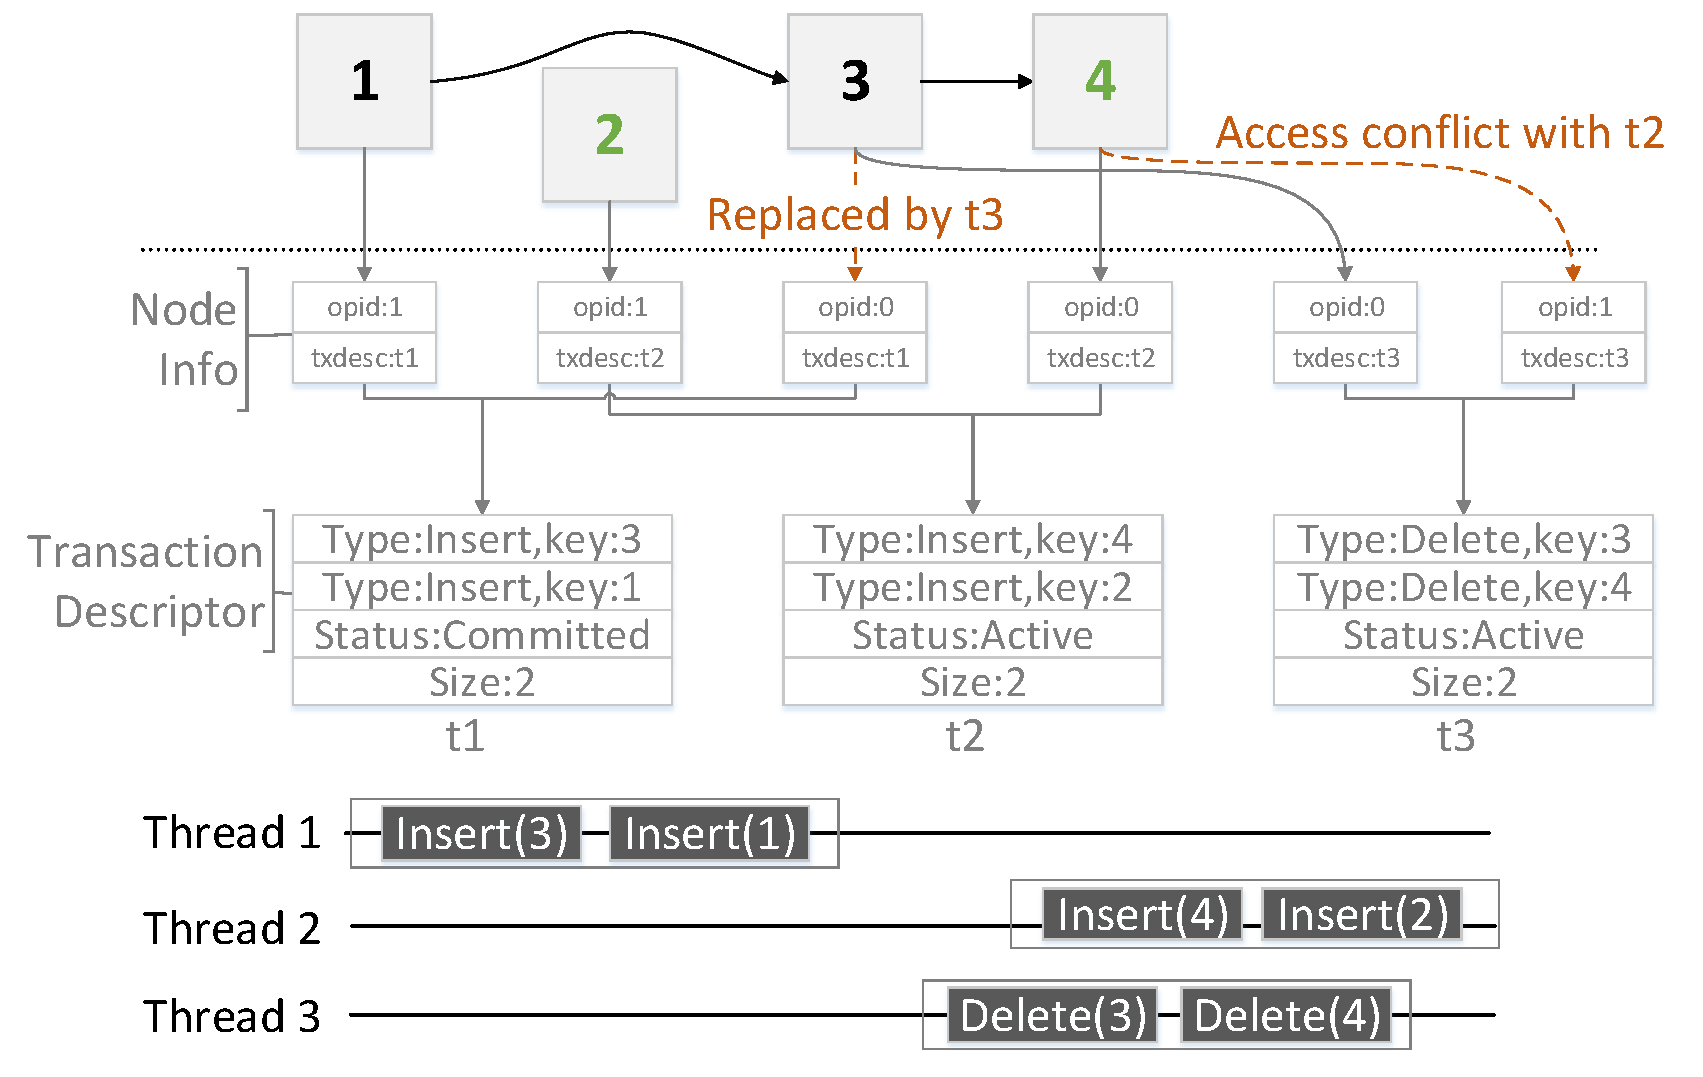
\includegraphics[width=1\columnwidth]{figure/lfttconflict.pdf}
    \caption{Transaction Execution and Conflict}
    \label{fig:lfttconflict}
\end{figure}

We illustrate an example of node access conflict in Figure~\ref{fig:lfttconflict}.
At the beginning, Thread 1 committed a transaction $t1$ inserting keys 1 and 3. 
Thread 2 attempted to insert keys 4 and 2 in transaction $t2$, while Thread 3 was concurrently executing transaction $t3$ to delete keys 3 and 4.
Thread 3 was able to perform its first operation by updating the $info$ pointer on node 3 with a new \textsc{NodeInfo}.
However, it encounters a conflict when attempting to update node 4 because Thread 2 has yet to finish its second operation.
To enforce serialization, operations must not modify an active node. 
In order to guarantee lock-free progress, the later transaction must help carry out the remaining operations in the other active transaction.

Our synchronization protocol is \emph{pessimistic} in that it assigns a node to a transaction as soon as an operation requires it, for the duration of the transaction.
Moreover, node-based conflict detection effectively compartmentalizes the execution of transactions.
Completed operations will not be affected should a later operation in the transaction experience contention and need to retry (most lock-free data structures use CAS-based retry loops). 
Each node acts as a checkpoint; once an operation successfully updates a node, the transaction advances one step towards completion.  %permanently advances one step towards completion.
Data-based conflict detection, due to the lack of such algorithm-specific knowledge, has to restart the whole transaction upon conflict. 

\subsection{Logical Status Interpretation}
\label{sec:logical}
To achieve isolation in transaction executions, a write operation needs to buffer or ``hide'' its update until the transaction commits; and to achieve atomicity it needs to revoke its modifications upon transaction abort.
%Transactional boosting employs locks to ensure the former condition is met and it uses undo logs to rollback aborted transactions. 
In the context of data structure transactions, existing strategies undo the operations by invoking their inverse operations~\cite{herlihy2008transactional}.
This would incur a significant penalty because the compute cycles spent on the inverse operations do not contribute to the overall throughput and introduce additional contention.
We approach the recovery task from another angle: an aborted transaction does not need to physically invoke the inverse methods; executed operations in an aborted transaction just need to \emph{appear to have be undone}.
We achieve this by having operations \emph{inversely interpret} the logical status of nodes accessed by operations in an aborted transaction.
Both physical undo and our logical undo reach the same goal of restoring the abstract state of the data structure. 

\begin{algorithm}[t]
        %TODO: use the following line for function calls
        %\IsNodePresent{$\textbf{Node*}\; n,\; \textbf{int}\; key$}\;

        \SetKwFunction{IsNodePresent}{IsNodePresent}
        \SetKwProg{Function}{Function}{}{end}
        \Function(){\IsNodePresent{$\textbf{Node*}\; n,\; \textbf{int}\; key$}}{
	        \KwRet{ $n.key = key$ \label{l:nodeexist}}
	    } %TODO: something like this with the while loop labels
		\;
		\SetKwFunction{IsKeyPresent}{IsKeyPresent}
        \Function{\IsKeyPresent{$\textbf{NodeInfo*}\;info,\;\textbf{Desc*} desc$}}{
        $\textbf{OpType}\;op\gets info.desc.ops[info.opid]$\;
         $\textbf{TxStatus}\;status \gets info.desc.status$ \label{l:readoldstatus}\;
        \Switch{$status$} {
        	\uCase{$Active$}{
        		\If{$info.desc = desc$}{
        			\KwRet{ $op=Find \;\textbf{or}\; op=Insert$}\;
        		}
        		\Else{
        			\KwRet{ $op=Find \;\textbf{or}\; op=Delete$}\;
        		}
        	}
        	\uCase{$Committed$}{
        		\KwRet{ $op=Find \;\textbf{or}\; op=Insert$}
        	}
        	\Case{$Aborted$}{
        		\KwRet{ $op=Find \;\textbf{or}\; op=Find$}
        	}
        }
        \caption{Logical Status}
        \label{alg:logicalstatus}
		}       
\end{algorithm}

%\begin{algorithm}[t]
%	\SetKwFunction{IsNodePresent}{$\textbf{Node*}\; n,\; \textbf{int}\; key$}
%	\KwRet{ $n.key = key$ \label{l:nodeexist}} %TODO: something like this with the while loop labels
%	
%	\SetKwFunction{IsKeyPresent}{$\textbf{NodeInfo*}\;info,\textbf{Desc*} desc$}
%	\ $\textbf{OpType}\;op\gets info.desc.ops[info.opid]$
%	$\textbf{TxStatus}\;status \gets info.desc.status$ \label{l:readoldstatus}
%	$\textbf{switch}\;${$status$} 
%	$\textbf{case:}\;${$\textbf{active}$}
%	$\textbf{if}$ {$info.desc=desc$} $\textbf{then}$
%	\KwRet{ $op=\textbf{find} \;\textbf{or}\; op=\textbf{insert}$}
%	$\textbf{else}$
%	\KwRet{ $op=\textbf{find} \;\textbf{or}\; op=\textbf{delete}$ }
%	%endif
%	
%	$\textbf{case:}\;${$\textbf{committed}$} 
%	\KwRet{ $op=\textbf{find} \;\textbf{or}\; op=\textbf{insert}$}
%	
%	$\textbf{case:}\;${$\textbf{aborted}$}
%	\KwRet{ $op=\textbf{find} \;\textbf{or}\; op=\textbf{delete}$}
%	\caption{Logical Status}
%	\label{alg:logicalstatus}          
%\end{algorithm}

\begin{algorithm}[t]
	\SetKwFunction{UpdateInfo}{UpdateInfo}
	\SetKwProg{Function}{Function}{}{end}
	\Function{\UpdateInfo{$\textbf{Node*}\;n,\;\textbf{NodeInfo*}\;info,\;$ $\textbf{bool}\;wantkey$}}{
		$\textbf{NodeInfo*}\; oldinfo \gets n.info$\; \label{l:readinfo}
		\If{$\textsc{IsMarked}(oldinfo)$}{
			$\textsc{Do\_Delete}(n)$\;
			\KwRet{ retry}
		}
		\If{$oldinfo.desc \neq info.desc$}{ \label{l:testself}
			\textsc{ExecuteOps}($oldinfo.desc,\;oldinfo.opid + 1$) \label{l:helpops}
		}
		\ElseIf{$oldinfo.desc,\;oldinfo.opid + 1$}{ \label{l:testhelped}
			\KwRet{ success}
		}
		$\textbf{bool}\;haskey \gets \textsc{IsKeyPresent}(oldinfo)$ \label{l:testkey} \;
		\If{$(!haskey \;\textbf{and}\; wantkey) \;\textbf{or}\; (haskey \;\textbf{and}\; !wantkey)$}{ \label{l:testdesire}
			\KwRet{ fail \label{l:infofail1}}
		}
		\If{$info.desc.status \neq Active$}{ \label{l:testactive}
			\KwRet{ fail \label{l:infofail2}}
		}
		\If{\textsc{CAS}$(\&n.info,\;oldinfo,\;info)$}{ \label{l:casinfo}
			\KwRet{ success}
		}
		\Else{
			\KwRet{ retry}
		}
	}
    \caption{Update NodeInfo}
    \label{alg:updateinfo}
\end{algorithm}


In Algorithm~\ref{alg:logicalstatus}, we list the function to interpret the logical status of a node according to the value of the transaction descriptor.
Function \textsc{IsNodePresent}, verifies that a node associated with a specific key is present.
This is a common test found in existing linked data structures.
Given a node's presence, function \textsc{IsKeyPresent} verifies if the key should be logically included in the abstract state, and returns a boolean value based on the combination of operation type and transaction status.
For a node most recently accessed by an \textsc{Insert} operation, its key is considered present if the transaction has successfully \emph{committed}.
On the contrary, according to the semantics of \textsc{Delete}, a successful operation must remove the key from the set.
Thus for a node most recently accessed by a \textsc{Delete} operation, its key is considered present if the transaction has \emph{aborted}.
These two opposite interpretations also match previous observations that \textsc{Insert} and \textsc{Delete} are a pair of inverse operations~\cite{herlihy2008transactional}.
Since the \textsc{Find} operation is read-only, no rollback is needed.
The node's key is always present regardless the status of the transaction.
A special case is the operations in an active transaction, which we treat as committed but are visible only to subsequent operations within the same transaction scope.
%Suppose a transaction contains two operations \textsc{Insert(4)} and \textsc{Find(4)}. The later needs to recognize the key newly inserted by the former as present. 

\begin{algorithm}[th]

    %\begin{algorithmic}[1]
         $\textbf{thread\_local\;Stack}\;helpstack$\;
         \SetKwFunction{ExecuteTransaction}{ExecuteTransaction}
         \SetKwProg{Function}{Function}{}{end}
         \Function{\ExecuteTransaction{$\textbf{Desc*}\;desc$}}{
         	$helpstack.\textsc{Init}()$ \label{l:stackinit} \;
         	$\textsc{ExecuteOps}(desc, 0)$\;
         	\KwRet{ $desc.status = Committed$}
         }
        \;
        
        \SetKwFunction{ExecuteOps}{ExecuteOps}
        \SetKwProg{Function}{Function}{}{end}
        \Function{\ExecuteOps{$\textbf{Desc*}\;desc,\;\textbf{int}\;opid$}}{
        	$\textbf{bool}\;ret \gets \textbf{true}$\;
        	$\textbf{set}\;delnodes$\;
        	\If{$helpstack.\textsc{Contains}(desc)$}{ \label{l:stackcontain}
        		$\text{\textsc{CAS}}(\&desc.flag,\;Active,\;Aborted)$ \label{l:txncyclicabort}\;
        		\KwRet{}
        	}
        	$helpstack.\textsc{Push}(desc)$ \label{l:stackpush} \;
        	\While {$desc.status = Active$ $\;\textbf{and}\; ret \;\textbf{and}\;$ $opid < desc.size$}{ \label{l:txnwhile}
        		$\textbf{Operation*}\;op \gets desc.ops[opid]$\;
        		\If{$op.type = \textbf{find}$}{
        			$ret \gets \textsc{Find}(op.key,\;desc,\;opid)$
        		}
        		\ElseIf{$op.type = Insert$}{
        			$ret \gets \textsc{Insert}(op.key,\;desc,\;opid)$
        		}
        		\ElseIf{$op.type = Delete$}{
        			$\textbf{Node*}\;del$\;
        			$ret \gets \textsc{Delete}(op.key,\;desc,\;opid,\;del)$\;
        			$delnodes.\textsc{Insert}(del)$
        		}
        		$opid \gets opid + 1$\;
        	}
        	$helpstack.\textsc{Pop}()$ \label{l:stackpop} \;
        	\If{$ret = \textbf{true}$}{
        		\If{$\text{\textsc{CAS}}(\&desc.flag,\;Active,\;Committed)$}{ \label{l:txnsuccess}
        			$\textsc{MarkDelete}(delnodes,\;desc)$ \label{l:markdelete}
        		}
        	}
        	\Else{
        		$\text{\textsc{CAS}}(\&desc.flag,\;Active,\;Aborted)$ \label{l:txnfail}
        	}
        }
        \caption{Transaction Execution}
        \label{alg:transaction}
\end{algorithm}

\subsection{Logical Status Update}
\label{sec:logicalupdate}
As mentioned above, the logical status of a node depends on the interpretation of its transaction descriptor. 
In a transformed data structure, an operation needs to change a node's logical status before performing any necessary low-level node manipulations. 
This is done by updating the node's \textsc{NodeInfo} pointer as shown in Algorithm~\ref{alg:updateinfo}. 
Given a node $n$, the function \textsc{UpdateInfo} reads its current $info$ field (line~\ref{alg:updateinfo}.\ref{l:readinfo}~\footnote{We denote line $b$ from algroithm $a$ by $a.b$}), verifies its sanity, and attempts to update $n.info$ through the use of CAS (line~\ref{alg:updateinfo}.\ref{l:casinfo}).
It returns a tri-state value indicating whether the operation succeeded, failed, or should be retried.
We make sure that any other active transaction accessing $n$ is completed by helping execute its remaining operations (line~\ref{alg:updateinfo}.\ref{l:helpops}).
%We explain the details of \textsc{ExecuteOps} in the next section.
However, we have to avoid helping the same transaction because of the hazard of infinite recursions.
This is prevented by the condition check on line~\ref{alg:updateinfo}.\ref{l:testself}.
We also skip the update and report success if the operation has already been performed by other threads (line~\ref{alg:updateinfo}.\ref{l:testhelped}).
Due to the use of the helping mechanism, the same operation may be executed multiple times by different threads.
The condition check on line~\ref{alg:updateinfo}.\ref{l:testhelped} allows us to identify the node accessed by threads that execute the same transaction, and ensures consistent results.
We validate the presence of the key on line~\ref{alg:updateinfo}.\ref{l:testkey} and test if the key's presence (as required by deletions and finds), or lack of presence (as required by insertions), is desired on line~\ref{alg:updateinfo}.\ref{l:testdesire}. The boolean flag $wantkey$ is passed on by the caller function to indicate if the presence of key is desired.
The operation reports failure when $wantkey$ contradicts $haskey$.
Finally, we validate that the transaction is still active (line~\ref{alg:updateinfo}.\ref{l:testactive}) to prevent a terminated transaction from erroneously overwriting $n.info$.

\subsection{Transaction Execution}
\label{sec:txnexec}
We consider the transaction execution model in which a transaction explicitly aborts upon the first operation failure.
The \textsc{ExecuteTransaction} in Algorithm~\ref{alg:transaction} is the entry point of transaction execution, which is invoked by the thread that initiates a transaction.
The \textsc{ExecuteOps} function executes operations in sequence starting from $opid$.
For threads that help to execute a delayed transaction, the $opid$ could be in the range of $[1,\;desc.size]$.
In each step of the while loop (line~\ref{alg:transaction}.\ref{l:txnwhile}), the return value of the previous operation is verified.
We require the operations to return a boolean value indicating if the executions are successful.
A false value indicates the precondition required by the operation is unsatisfied and the transaction will abort. 
Once all operations complete successfully we atomically update the transaction status with a \emph{Committed} flag (line~\ref{alg:transaction}.\ref{l:txnsuccess}).
It is not necessary to retry this CAS operation as a failed CAS indicates that some other thread must have successfully updated the transaction status.
The thread that successfully executed the CAS will be responsible for performing physical node deletion (line~\ref{alg:transaction}.\ref{l:markdelete}), which will be explained in Section~\ref{sec:application}.

By adopting cooperative transaction execution, our approach is able to eliminate the majority of aborts caused by access conflicts.
Although rare, potential livelock is possible if two threads were to access two of the same nodes in opposite order.
In such cases, both threads will be trapped in infinite recursions helping execute each other's transaction.
We detect and recover from this hazard by using a per-thread \emph{help stack}, which is a simple stack containing $Desc$ pointers. 
This is similar to a function call stack, except it records the invocation of \textsc{ExecuteOps}.
A thread initializes its help stack before initiating a transaction.
Each time a thread begins to help another transaction, it pushes the transaction descriptor onto its help stack.
A thread pops its help stack once the help completes.
Cyclic dependencies among transactions can be detected by checking for duplicate entries in the help stack (line~\ref{alg:transaction}.\ref{l:stackcontain}). 
We recover by aborting one of the transactions as shown on line~\ref{alg:transaction}.\ref{l:txncyclicabort}.

\begin{algorithm}[t]
	\SetKwFunction{UpdateInfo}{UpdateInfo}
	\SetKwProg{Function}{Function}{}{end}
	\Function{\UpdateInfo{$\textbf{Node*}\;n,\;\textbf{NodeInfo*}\;info,\;$ $\textbf{bool}\;wantkey$}}{
		$\textbf{NodeInfo*}\; oldinfo \gets n.info$\;
		\If{$\textsc{IsMarked}(oldinfo)$}{
			$\textsc{Do\_Delete}(n)$\;
			\KwRet{ retry}
		}
		\If{$oldinfo.desc \neq info.desc$}{ \label{l:obstestself}
			$\textsc{CAS}(\&oldInfo.desc,\;Active,\;Aborted)$ \label{l:abortcompetitor}
		}
		\ElseIf{$oldinfo.desc,\;oldinfo.opid + 1$}{
			\KwRet{ success}
		}
		$\textbf{bool}\;haskey \gets \textsc{IsKeyPresent}(oldinfo)$ \;
		\If{$(!haskey \;\textbf{and}\; wantkey) \;\textbf{or}\; (haskey \;\textbf{and}\; !wantkey)$}{
			\KwRet{ fail }
		}
		\If{$info.desc.status \neq Active$}{
			\KwRet{ fail }
		}
		\If{$\textsc{CAS}(\&n.info,\;oldinfo,\;info)$}{
			\KwRet{ success}
		}
		\Else{
			\KwRet{ retry}
		}
	}
	\caption{Obstruction-free Update NodeInfo}
	\label{alg:obstructionfreeupdateinfo}
\end{algorithm}

\begin{algorithm}[th]
	
	%\begin{algorithmic}[1]
	\SetKwFunction{ExecuteTransaction}{ExecuteTransaction}
	\SetKwProg{Function}{Function}{}{end}
	\Function{\ExecuteTransaction{$\textbf{Desc*}\;desc$}}{
		$\textsc{ExecuteOps}(desc, 0)$\;
		\KwRet{ $desc.status = Committed$}
	}
	\;
	
	\SetKwFunction{ExecuteOps}{ExecuteOps}
	\SetKwProg{Function}{Function}{}{end}
	\Function{\ExecuteOps{$\textbf{Desc*}\;desc,\;\textbf{int}\;opid$}}{
		$\textbf{bool}\;ret \gets \textbf{true}$\;
		$\textbf{set}\;delnodes$\;
		\While {$desc.status = Active$ $\;\textbf{and}\; ret \;\textbf{and}\;$ $opid < desc.size$}{
			$\textbf{Operation*}\;op \gets desc.ops[opid]$\;
			\If{$op.type = \textbf{find}$}{
				$ret \gets \textsc{Find}(op.key,\;desc,\;opid)$
			}
			\ElseIf{$op.type = Insert$}{
				$ret \gets \textsc{Insert}(op.key,\;desc,\;opid)$
			}
			\ElseIf{$op.type = Delete$}{
				$\textbf{Node*}\;del$\;
				$ret \gets \textsc{Delete}(op.key,\;desc,\;opid,\;del)$\;
				$delnodes.\textsc{Insert}(del)$
			}
			$opid \gets opid + 1$\;
		}
		\If{$ret = \textbf{true}$}{
			\If{$\text{\textsc{CAS}}(\&desc.flag,\;Active,\;Committed)$}{
				$\textsc{MarkDelete}(delnodes,\;desc)$
			}
		}
		\Else{
			$\text{\textsc{CAS}}(\&desc.flag,\;Active,\;Aborted)$
		}
	}
	\caption{Obstruction-free Transaction Execution}
	\label{alg:obstructionfreetransaction}
\end{algorithm}

\subsection{Obstruction-free Approach}
Our cooperative contention management strategy requires that the users specify all operations in a transaction beforehand.
However, some applications would benefit from dynamic transaction execution, in which the operations in a transaction are not pre-determined prior to the execution of the transaction.
In these applications, after a transaction begins, the operation types or operands of future method calls may depend on user input or other external events.
Our helping scheme could possibly support dynamic transaction execution, but it would break the data structure's lock-free progress guarantee.
For example, consider one transaction that begins by modifying node $n$ and then waits on user input for its next operation.
Other concurrent transactions that access $n$ need to help that transaction before performing their own operations on $n$.
This causes the concurrent transactions to be blocked (waiting on the user input) even though their own operations do not require user input.

To allow dynamic transaction execution, we introduce an alternative approach called obstruction-free transactional transformation, which eliminates the helping mechanism of the original lock-free approach.
It instead adopts an aggressive contention management strategy.
When two transactions conflict, the later transaction forcibly aborts the earlier one.
In the previous example, the transaction that is waiting on user input may be aborted by concurrent transactions, causing it to restart.
This allows the concurrent transactions to continue with their own operations without needlessly waiting on user input.
In this case, the progress guarantee provided by the system degrades to obstruction-free.
Obstruction-freedom guarantees that if a method executes without interruption from other threads, then it will finish in a finite number of steps.

Other contention management strategies are possible, such as having the thread can also abort itself, or aborting the transaction that has fewer completed operations.
We can apply a large number of contention management scheme that are currently adopted by STMs.
We chose aggressive contention management in our case, as it is able to demonstrate the idea of obstruction-free execution without the clutter of complex contention management algorithms.

We modify the lock-free \textsc{UpdateInfo} function shown in Algorithm~\ref{alg:updateinfo} to produce the obstruction-free \textsc{UpdateInfo} function listed in Algorithm~\ref{alg:obstructionfreeupdateinfo}.
In both versions, a transaction examines the target node $n$ to check if a conflicting transaction is also accessing $n$ (line~\ref{alg:updateinfo}.\ref{l:testself} and line~\ref{alg:obstructionfreeupdateinfo}.\ref{l:obstestself}).
If so, a contention management strategy must be applied to ensure serializability.
The lock-free version helps the conflicting transaction by executing that transaction's operations (line~\ref{alg:updateinfo}.\ref{l:helpops}).
The obstruction-free version instead aborts the conflicting transaction if it is still active (line~\ref{alg:obstructionfreeupdateinfo}.\ref{l:abortcompetitor}).

We modify the methods dealing with transaction execution shown in Algorithm~\ref{alg:transaction} to produce the obstruction-free methods listed in Algorithm~\ref{alg:obstructionfreetransaction}.
Because the helping mechanism can cause cyclic dependencies between transactions, the lock-free version must create and maintain a thread-local \emph{help stack}, which contains the descriptors of the transactions that the thread is currently helping.
Cyclic dependencies are detected by checking for duplicate transaction descriptors in the help stack (line~\ref{alg:transaction}.\ref{l:stackcontain}).
The obstruction-free approach does not allow such cyclic dependencies to occur, so we remove the help stack.


\section{Application Examples}
\label{sec:application}
In this section, we present the application of our methodology to linked lists and skiplists, and hash maps.

\subsection{Linked List and Skiplist Based Sets}
\label{sec:lists}
In this section, we demonstrate the application of our lock-free transaction transformation on linked list and skiplist based sets. 
The process involves two steps: 1) identify and encapsulate the base data structure's methods for locating, inserting, and deleting nodes; and 2) integrate the \textsc{UpdateInfo} function (Algorithm~\ref{alg:updateinfo}) in each operation using the templates provided in this section.

The first step is necessary because we still rely on the base algorithm and its concurrency control to add, update, and remove linkage among nodes.
This is a refactoring process, as we do not alter the functionality of the base implementations. 
Although implementation details such as argument types and return values may vary, we need to extract the following three functions: \textsc{Do\_LocatePred}, \textsc{Do\_Insert}, and \textsc{Do\_Delete}.
We add a prefix \textsc{Do\_} to indicate these are the methods provided by the base data structures.
For brevity, we omit detailed code listings, but express the general functionality specifications.
Given a key, \textsc{Do\_LocatePred} returns the target node (and any necessary variables for linking and unlinking a node, e.g., its predecessor).
\textsc{Do\_Insert} creates the necessary linkage to correctly place the new node in the data structure.
\textsc{Do\_Delete} removes any references to the node.
Note that some lock-free data structures~\cite{harris2001pragmatic,fraser2004practical} employ a two-phased deletion algorithm, where the actual node removal is delayed or even separated from the first phase of logical deletion.
In this case, we only expect \textsc{Do\_Delete} to perform the logical deletion as nodes will be physically removed during the next traversal.
%We also assume there will be sentinel head and tail nodes so that the \textsc{Do\_LocatePred} function will not return null pointers.

Algorithm~\ref{alg:listinsert} lists the template for the transformed \textsc{Insert} function.
The function resembles the base node insertion algorithm with a CAS-based while loop (line~\ref{alg:listinsert}.\ref{l:listinsertwhile}).
The only addition is the code path for invoking \textsc{UpdateInfo} on line~\ref{alg:listinsert}.\ref{l:insupdateinfo}.
The logic is simple: on line~\ref{alg:listinsert}.\ref{l:listinsertcontain} we check if the data structure already contains a node with the target key.
If so, we try to update the node's logical status, otherwise we fall back to the base code path to insert a new node. 
Should any of the two code paths indicate a retry due to contention, we start the traversal over again.

\begin{algorithm}[t]

    %\begin{algorithmic}[1]
	\SetKwFunction{Insert}{Insert}
	\SetKwProg{Function}{Function}{}{end}
	\Function{\Insert{$\textbf{int}\;key,\;\textbf{Desc*}\;desc,\;\textbf{int}\;opid$}}{
    	$\textbf{NodeInfo*}\; info \gets \text{\textbf{new NodeInfo}}$\;
    	$info.desc \gets desc,\;info.opid \gets opid$\;
    	\While{\textbf{true}}{ \label{l:listinsertwhile}
    		$\textbf{Node*}\;curr \gets \textsc{Do\_LocatePred}(key)$\;
    		\If{$\textsc{IsNodePresent}(curr,\;key)$}{ \label{l:listinsertcontain}
    			$ret \gets \textsc{UpdateInfo}(curr,\;info,\;false)$ \label{l:insupdateinfo}
    		}
    		\Else{
    			$\textbf{Node*}\; n \gets \text{\textbf{new Node}}$\;
    			$n.key \gets key,\;n.info \gets info$\;
    			$ret \gets \textsc{Do\_Insert}(n)$ \label{l:linknode}
    		}
    		\If{$ret = success$}{
    			\KwRet{ \textbf{true}}
    		}
    		\ElseIf{$ret = fail$}{
    			\KwRet{ \textbf{false}}
    		}
    	}
	}
    %\end{algorithmic}
        \caption{Template for Transformed Insert Function}
        \label{alg:listinsert}
\end{algorithm}

\begin{algorithm}[t]

	\SetKwFunction{Find}{Find}
	\SetKwProg{Function}{Function}{}{end}
	\Function{\Find{$\textbf{int}\;key,\;\textbf{Desc*}\;desc,\;\textbf{int}\;opid$}}{
		$\textbf{NodeInfo*}\; info \gets \text{\textbf{new NodeInfo}}$\;
		$info.desc \gets desc,\;info.opid \gets opid$\;
		\While{\textbf{true}}{ \label{l:listinsertwhile}
			$\textbf{Node*}\;curr \gets \textsc{Do\_LocatePred}(key)$\;
			\If{\textsc{IsNodePresent}($curr,\;key$)}{ \label{l:listinsertcontain}
				$ret \gets \textsc{UpdateInfo}(curr,\;info,\;true)$ \label{l:insupdateinfo}
			}
			\Else{
				$ret \gets fail$ \label{l:linknode}
			}
			\If{$ret = success$}{
				\KwRet{ \textbf{true}}
			}
			\ElseIf{$ret = fail$}{ \label{l:findfail}
				\KwRet{ \textbf{false}}
			}
		}
	}
    %\end{algorithmic}
        \caption{Template for Transformed Find Function}
        \label{alg:listfind}
\end{algorithm}

\begin{algorithm}[h]

	\SetKwFunction{Delete}{Delete}
	\SetKwProg{Function}{Function}{}{end}
	\Function{\Delete{$\textbf{int}\;key,\;\textbf{Desc*}\;desc,\;\textbf{int}\;opid$}}{
		$\textbf{NodeInfo*}\; info \gets \text{\textbf{new NodeInfo}}$\;
		$info.desc \gets desc,\;info.opid \gets opid$\;
		\While{\textbf{true}}{ \label{l:listinsertwhile}
			$\textbf{Node*}\;curr \gets \textsc{Do\_LocatePred}(key)$\;
			\If{\textsc{IsNodePresent}($curr,\;key$)}{ \label{l:listinsertcontain}
				$ret \gets \textsc{UpdateInfo}(curr,\;info,\;true)$ \label{l:insupdateinfo}
			}
			\Else{
				$ret \gets fail$ \label{l:linknode}
			}
			\If{$ret = success$}{
				$del \gets curr$\;
				\KwRet{ \textbf{true}}
			}
			\ElseIf{$ret = fail$}{ \label{l:deletefail}
				$del \gets NIL$\;
				\KwRet{ \textbf{false}}
			}
		}
	}
	\;
	
	\SetKwFunction{MarkDelete}{MarkDelete}
	\SetKwProg{Function}{Function}{}{end}
	\Function{\MarkDelete{$\textbf{set}\;delnodes,\;\textbf{Desc*}\;desc$}}{
		\For {$del \in delnodes$}{
			\If{$del = NIL$}{
				\textbf{continue}
			}
			$\textbf{NodeInfo*}\;info \gets del.info$\;
			\If{$info.desc \ne desc$}{
				\textbf{continue}
			}
			\If{$\textsc{CAS}(del.info,\;info,\;\textsc{SetMark}(info))$}{ \label{l:markinfo}
				$\textsc{Do\_Delete}(del)$
			}
		}
	}
        \caption{Template for Transformed Delete Function}
        \label{alg:listdelete}
\end{algorithm}


The \textsc{Delete} operation listed in Algorithm~\ref{alg:listdelete} is identical to \textsc{Insert} except it terminates with failure when the target node does not exist (line~\ref{alg:listdelete}.\ref{l:deletefail}).
We also adopt a two-phase process for unlinking nodes from the data structure: deleted nodes will firstly be buffered in a local set in \textsc{ExecuteOps}, and when the transaction commits, the $info$ field of buffered nodes will be marked (line~\ref{alg:listdelete}.\ref{l:markinfo}) and consequently unlinked from the data structure by invoking the base data structures' \textsc{Do\_Delete}.
One advantage of our logical status interpretation is that unlinking nodes from the data structure is optional, whereas in transactional boosting nodes must be physically unlinked to restore the abstract state. 
This opens up opportunities to optimize performance based on application scenarios.
Timely unlinking deleted nodes is important for linked lists because the number of ``zombie'' nodes has linear impact on sequential search time.
Leaving delete nodes in the data structure may be beneficial for skiplists because the overhead and contention introduced by unlinking nodes may outweigh the slight increase in sequential search time ($\mathcal{O}(log{}n)$).

The \textsc{Find} operation listed in Algorithm~\ref{alg:listfind} also needs to update the node's $info$ pointer.
Without this, concurrent deletions may remove the node after \textsc{Find} has returned and before the transaction commits.
%Our \textsc{Find} operation is not literally read-only anymore, but it still is in the logical sense.
Since we have extracted the core functionality of interpreting and updating logical status into a common subroutine, the transformation process is generic and straightforward.
To use a transformed data structure, the application should first initialize and fill a \textsc{Desc} structure, then invoke \textsc{ExecuteTransaction} (Algorithm~\ref{alg:transaction}) with it as an argument.
The allocation of the transaction descriptor contributes to most of the transaction execution overhead.
We discuss this in more details in Section~\ref{sec:experiment}.

\subsection{Hash Maps}
\label{sec:maps}
In this section, we demonstrate the application of our lock-free transaction transformation on hash maps.
Map data structures store keys and their associated values.
Maps also provide an update operation to change the value associated with a particular key, in addition to the insert, find, and remove operations that are present in set data structures.
To support map data structures we add a \textsc{value} field to the \textsc{Operation} and \textsc{Node} structs present in Algorithm~\ref{alg:nodestructure}, and an \textsc{Update} to the \textsc{OpType} enumeration.

The reason we make these changes to Algorithm~\ref{alg:nodestructure} is to provide two different places to save a node's value, one in the node itself, and one in the node's descriptor.
We use these two locations to preserve the current value of a node, and buffer pending updates in the node's descriptor.
This allows \textsc{Find} operations from the same transaction to return the correct \textsc{value}, held in the descriptor, if the transaction commits, without erroneously overwriting the value stored in the node by the most recently committed transaction.
If we use the \textsc{Find} operation from Algorithm~\ref{alg:listfind}, we will erroneously overwrite pending updates as the \textsc{Find} operation will place its descriptor at a node, overwriting the node descriptor of the active \textsc{Update} operation.
To solve this problem, we note that the node descriptor of a \textsc{Find} operation only needs to store the key that it is searching for, and its operation type.
In this case, the pending update can be preserved by copying its value from the old node descriptor of the \textsc{Update} operation to the node descriptor of the \textsc{Find} operation which is now placed at the node.
In this way, the pending writes to a node's value can be preserved without overwriting the node's current value, which would prevent inverse interpretation on transaction abort.
This is an extension of logical status interpretation, as we choose a different \textsc{value} depending on whether or not the transaction is \textsc{aborted}, \textsc{active}, or \textsc{committed}.

Our changes to Algorithm~\ref{alg:nodestructure} allow us to perform logical status interpretation on key-value pairs as we will be able to recover the previous value associated with a key if an \textsc{Update} operation is aborted.
We propagate this change to \textsc{IsKeyPresent} by treating the \textsc{Update} operation the same way we treat a \textsc{Find}, as neither operation changes the presence of a key.

To perform logical status interpretation of a key-value pair we implement an \textsc{IsValuePresent} function as the \textsc{Update} operation buffers writes to a node in the node's descriptor until it commits.
The pseudocode for this function is presented in Algorithm~\ref{alg:maplogicalstatus}.
This function returns whether or not the value present in the \textsc{Node} should be treated as present; if not, the value in the \textsc{NodeInfo} descriptor is used, because there is a pending update from the same transaction descriptor whose buffered write is logically interpreted as the node's value.

In the \textsc{IsValuePresent} function, \textsc{INVALID} represents a sentinel value that indicates a value has not been set for a \textsc{Find} operation.
The semantics that we adhere to for a map data structure do not allow the user to search for a specific key-value pair, instead the user searches for a key and the matching value is returned.
We use the \textsc{value} field of a \textsc{Find} operation to hold pending updates buffered in a node's descriptor which would otherwise be erroneously overwritten by \textsc{Find} placing its own \textsc{NodeInfo} descriptor at that node.

We copy the pending updates, which are buffered in a node's descriptor, to the node in a lazy fashion.
Once the transaction with the pending updates is committed, the next \textsc{Find} or \textsc{Update} operation that attempts to update the \textsc{NodeInfo} descriptor of that node will examine that node descriptor in order to determine whether or not the last operation that was performed was a committed \textsc{Find} or \textsc{Update}.
If it sees a \textsc{Find} operation's descriptor that holds a different valid \textsc{value} from the one currently stored in the node, one that is not equal to the sentinel \textsc{INVALID}, then the \textsc{MapUpdateInfo} algorithm will store that value as the node's value.
If the operation sees an \textsc{Update} descriptor at the node, with any value other than that currently stored in the node, then the operation copies the value stored in the descriptor to the node.
Once the operation completes the copy, it can perform its operation as usual.
This copy preserves correct semantics for all operations, as the old \textsc{value} will be ignored by an \textsc{Insert} or \textsc{Delete} operation, and a \textsc{Find} or \textsc{Update} operation uses the new value in the node's \textsc{value} field.
The pseudocode for the \textsc{MapUpdateInfo} algorithm is displayed in Algorithm~\ref{alg:mapupdateinfo}.
The lazy update of the node's value occurs in the if-then statement on line~\ref{alg:mapupdateinfo}.\ref{l:isunsaved}.

%We update the \textsc{UpdateInfo} function presented in Algorithm~\ref{alg:updateinfo} to use the buffered write operations when they are logically present in a node's descriptor, in Algorithm~\ref{alg:mapupdateinfo}.


\begin{algorithm}[t]
	%TODO: use the following line for function calls
	%\IsNodePresent{$\textbf{Node*}\; n,\; \textbf{int}\; key$}\;
	
	\SetKwFunction{IsNodePresent}{IsNodePresent}
	\SetKwProg{Function}{Function}{}{end}
	\Function(){\IsNodePresent{$\textbf{Node*}\; n,\; \textbf{int}\; key$}}{
		\KwRet{ $n.key = key$ }
	} %TODO: something like this with the while loop labels
	\;
	\SetKwFunction{IsKeyPresent}{IsKeyPresent}
	\Function{\IsKeyPresent{$\textbf{NodeInfo*}\;info,\;\textbf{Desc*} desc$}}{
		$\textbf{OpType}\;op\gets info.desc.ops[info.opid]$\;
		$\textbf{TxStatus}\;status \gets info.desc.status$\;
		\Switch{$status$} {
			\uCase{$Active$}{
				\If{$info.desc = desc$}{
					\KwRet{ $op=Update \;\textbf{or}\; op=Find \;\textbf{or}\; op=Insert$}\;
				}
				\Else{
					\KwRet{ $op=Update \;\textbf{or}\; op=Find \;\textbf{or}\; op=Delete$}\;
				}
			}
			\uCase{$Committed$}{
				\KwRet{ $op=Update \;\textbf{or}\; op=Find \;\textbf{or}\; op=Insert$}
			}
			\Case{$Aborted$}{
				\KwRet{ $op=Update \;\textbf{or}\; op=Find \;\textbf{or}\; op=Find$}
			}
		}
	}
	\;
	\SetKwFunction{IsValuePresent}{IsValuePresent}
	\Function{\IsValuePresent{$\textbf{NodeInfo*}\;info$}}{
		$\textbf{Operation}\;op\gets info.desc.ops[info.opid]$\;
		\If{$op.type == Update\; ||\; op.type == Find \;\&\&\; op.value != \text{INVALID}$}{
			$return\;false$\;
		}
		$return\;true$\;
	}
	\caption{Logical Status for Maps}
	\label{alg:maplogicalstatus}
\end{algorithm}

As with the transactional linked list and skiplist, we encapsulate the base data structure's methods for locating, inserting, and deleting nodes.
We describe the templates for each of the four canonical map operations \textsc{Insert}, \textsc{Delete}, \textsc{Find}, and \textsc{Update}.
The only change we make to the templates for the \textsc{Insert}, \textsc{Delete}, and \textsc{Find} operations as shown in Algorithms~\ref{alg:listinsert},~\ref{alg:listdelete}, and~\ref{alg:listfind} is that we must set the \textsc{value} field of the new node in an \textsc{Insert} to the value that is associated with the key.
No other changes are necessary as these operations do not examine the value associated with a key.
Additionally, the underlying \textsc{LocatePred} algorithm must search for a node using the hashed key instead of the key itself.
The template for the \textsc{Update} function is similar to that of the \textsc{Insert} function (except we call \textsc{MapUpdateInfo} with \textsc{true} as the final argument), since the \textsc{MapUpdateInfo} function lazily updates the \textsc{value} of a node.

\begin{algorithm}[t]
	\SetKwFunction{MapUpdateInfo}{MapUpdateInfo}
	\SetKwProg{Function}{Function}{}{end}
	\Function{\MapUpdateInfo{$\textbf{NodeInfo*}\;info,\;$ $\textbf{bool}\;wantkey$}}{
		$\textbf{NodeInfo*}\; oldinfo \gets n.info$\;
		\If{$\textsc{IsMarked}(oldinfo)$}{
			$\textsc{Do\_Delete}(n)$\;
			\KwRet{ retry}
		}
		\If{$oldinfo.desc \neq info.desc$}{
			\textsc{ExecuteOps}($oldinfo.desc,\;oldinfo.opid + 1$)
		}
		\ElseIf{$oldinfo.desc,\;oldinfo.opid + 1$}{
			\KwRet{ success}
		}
		$\textbf{bool}\;haskey \gets \textsc{IsKeyPresent}(oldinfo)$  \;
		\If{$(!haskey \;\textbf{and}\; wantkey) \;\textbf{or}\; (haskey \;\textbf{and}\; !wantkey)$}{ 
			\KwRet{ fail }
		}
		\If{$info.desc.status \neq Active$}{ 
			\KwRet{ fail }
		}
		$\textbf{Operation} op \gets info.desc.ops[info.opid]$\; \label{l:startUpdate}
		$\textbf{Operation}\; oldOp \gets oldinfo.desc.ops[oldinfo.opid]$\;
		\If{$op.type == Update \;||\; op.type == Find$}{ \label{l:isunsaved}
			\If{$oldOp.value \;!= \;node.value \;\&\& \;oldinfo.desc.status == Committed\; \&\&\; IsValuePresent(oldinfo)$}{
				$n.value \gets oldOp.value$\;
			}
		}
		
		\If{\textsc{CAS}$(\&n.info,\;oldinfo,\;info)$}{ 
			\If{$op.type \;==\; Find$}{
				\If{$oldOp.type \;==\; Update \;||\; (oldOp.type \;==\; Find \;\&\&\; oldOp.value \;!= \;INVALID)$}{
					$n.info.value \gets oldOp.value$\;
					\KwRet{$n.info.value$}\;
				}
				\Else{
					\KwRet{$n.value$}\;
				}
			}
			\KwRet{ success}
		}
		\Else{
			\KwRet{ retry}
		}
	}
	\caption{Update NodeInfo for Maps}
	\label{alg:mapupdateinfo}
\end{algorithm}
 

\section{Correctness}
\label{sec:correctness}
We base our correctness discussion on the notion of commutativity isolation~\cite{herlihy2008transactional}, which states that the history of committed transactions is \emph{strictly serializable} for any transactional data structure that provides linearizable operations and obeys commutativity isolation~\footnote{We omit the discussion of rules on compensating actions and disposable methods because they are not applicable to our approach}.
STM systems may prefer more strict correctness criteria, such as opacity~\cite{guerraoui2008correctness}, because they need to account for the consistency of intermediate memory access.
In the case of data structure transactions, the intermediate computation is managed by linearizable methods, and only the end result of a transaction is accessible to users.
Strict serializability~\cite{papadimitriou1979serializability}, which is the analogue of linearizability~\cite{herlihy1990linearizability} for transactions, provides enough semantics for such cases.

\subsection{Definitions}
We provide a brief recapitulation of the definitions and correctness rules from Herlihy and Koskinen's work~\cite{herlihy2008transactional}.
A \emph{history} of computation is a sequence of instantaneous events.
Events associated with a method call include invocation $I$ and response $R$.
%For a transaction, events associated with its status include $\langle T \textsf{ init} \rangle$, $\langle t \textsf{ commit} \rangle$, $\langle T \textsf{ abort} \rangle$ indicating $T$ start rolling back its effects, and $\langle T \textsf{ aborted} \rangle$ indicating $T$ finishes its rollback.
%We denote a sequence of events by concatenate them with $\cdot$: 
A single transaction running in isolation defines a \emph{sequential history}.
A \emph{sequential specification} for a data structure defines a set of \emph{legal histories} for that data structure.
%A \emph{concurrent history} is one in which events of different transactions are interleaved.
%A \emph{subhistory} is a subsequence of the events of $h$.
%The subhistory of $h$ restricted to transaction $T$ is denoted as $h|T$.
%The subhistory $committed(h)$ is the subsequence of $h$ consisting of all events of committed transactions.

\begin{definition}
    A history $h$ is strictly serializable if the subsequence of $h$ consisting of all events of committed transactions is equivalent to a legal history in which these transactions execute sequentially in the order they commit.
\end{definition}

%\begin{definition}
    %Histories $h$ and $h'$ define the same state if, for every history $g$, $h \cdot g$ is legal if and only if $h' \cdot g$ is.
%\end{definition}

%\begin{definition}
    %For a history $h$ and any given invocation $I$ and response $R$, let $I^{-1}$ and $R^{-1}$ be the \emph{inverse} invocation and response, such that the abstract state reached after the history $h \cdot I \cdot R \cdot I^{-1} \cdot R^{-1}$ is the same as the state reached after history $h$.
%\end{definition}

\begin{definition}
    Two method calls $I,R$ and $I',R'$ commute if: for all histories $h$, if $h \cdot I \cdot R$ and $h \cdot I' \cdot R'$ are both legal, then $h \cdot I \cdot R \cdot I' \cdot R'$ and $h \cdot I' \cdot R' \cdot I \cdot R$ are both legal and define the same abstract state.
\end{definition}

Commutativity identifies operations that have no dependencies on each other.
Executing commutative operations in any order yields the same abstract state.
The commutativity specification for set operations is as follows:
\begin{equation}
    \label{eq:commute}
\begin{aligned}
    \textsc{Insert}(x) \leftrightarrow \textsc{Insert}(y),\;x \ne y \\
    \textsc{Delete}(x) \leftrightarrow \textsc{Delete}(y),\;x \ne y \\
    \textsc{Insert}(x) \leftrightarrow \textsc{Delete}(y),\;x \ne y \\
    \textsc{Find}(x) \leftrightarrow \textsc{Insert}(x)/false \leftrightarrow \textsc{Delete}(x)/false
\end{aligned}
\end{equation}

\begin{crule}
    \textbf{Linearizability:} For any history $h$, two concurrent invocations $I$ and $I'$ must be equivalent to either the history $h \cdot I \cdot R \cdot I' \cdot R'$ or the history $h \cdot I' \cdot R' \cdot I \cdot R$
\end{crule}

\begin{crule}
    %TODO: non-commutative
    \textbf{Commutativity Isolation:} For any non-commut-ative method calls $I_1,R_1 \in T_1$ and $I_2,R_2 \in T_2$, either $T_1$ commits or aborts before any additional method calls in $T_2$ are invoked, or vice-versa.
\end{crule}

%\begin{crule}
    %\textbf{Compensating Actions:} For any history $h$ and transaction $T$, if $\langle T \textsf{ \textup{aborted}} \rangle \in h$, then it must be the case that $h|T=\langle T \textsf{ \textup{init}} \rangle \cdot I_0 \cdot R_0 \cdots I_i \cdot R_i \cdot \langle T \textsf{ \textup{abort}} \rangle \cdot I_i^{-1} \cdot R_i^{-1} \cdots I_0^{-1} \cdot R_0^{-1} \cdot \langle T \textsf{ \textup{aborted}} \rangle$ where $i$ indexes the last successfully completed method call.
%\end{crule}

\subsection{Serializability and Recoverability}
We now show that lock-free transactional transformation meets the two above correctness requirements. 
We denote the concrete state of a set as an node set $N$.
At any time, the abstract state observed by transaction $T_i$ is $S_i = \{n.key\;|\;n \in N \land \textsc{IsKeyPresent}(n.info,\;desc_i)\}$, where $desc_i$ is the descriptor of $T_i$.

Linearizability requires that concurrent operations appear as if they took place instantaneously at some points between their invocations and responses.
We show the transformed operations are linearizable by identifying their \emph{linearization points}.
Additionally, we use the notion of decision points and state-read points to facilitate our reasoning. 
The decision point of an operation is defined as the atomic statement that finitely decides the result of an operation, i.e. independent of the result of any subsequent instruction after that point.
A state-read point is defined as the atomic statement where the state of the dictionary, which determines the outcome of the decision point, is read.
%Moreover, if we treat the execution of a transaction as an composed method then it is also linearizable in the sense that its effect is published in one atomic step.

\begin{lemma}
    \label{lemma:linearizable}
    The set operations \textsc{Insert}, \textsc{Delete}, and \textsc{Find} are linearizable.
\end{lemma}
\begin{proof}
    For the transformed \textsc{Insert} operation, the execution is divided into two code paths by the condition check on line~\ref{alg:listinsert}.\ref{l:listinsertcontain}.
    The code path on line~\ref{alg:listinsert}.\ref{l:insupdateinfo} updates the existing node's logical status.
    Note that if the operation reports failure on line~\ref{alg:updateinfo}.\ref{l:infofail1} and~\ref{alg:updateinfo}.\ref{l:infofail2}, no write operation will be performed to change the logical status of the node.
    The state-read point for the former case is when the previous transaction status is read from $oldinfo.desc.status$ on line~\ref{alg:logicalstatus}.\ref{l:readoldstatus}.
    The state-read point for the later case is when the current transaction status is read from $info.desc.status$ on line~\ref{alg:updateinfo}.\ref{l:testactive}.
    The abstract states $S'$ observed by all transactions immediately after the reads are unchanged, i.e., $\forall i, S'_i = S_i $.
    For a successful logical status update, the decision point for it to take effect is when the CAS operation on line~\ref{alg:updateinfo}.\ref{l:casinfo} succeeds.
    The abstract states $S'$ observed by the transactions $T_d$ executing this operation immediately after the CAS is $i=d \implies S'_i = S_i \cup n.key$.
    For all other transactions $i \ne d \implies S'_i = S_i$.
    In all cases, the update of abstract states conforms to the sequential specification of the insert operation.
    The code path for physically adding linkage to the new node (line~\ref{alg:listinsert}.\ref{l:linknode}) is linearizable because the corresponding \textsc{Do\_Insert} operation in the base data structure is linearizable.
    
    The same reasoning process applies to the transformed \textsc{Delete} and \textsc{Find} operations because they share the same logical status update procedure with \textsc{Insert}.
\end{proof}

The commutativity isolation rule prevents operations that are not commutative from being executed concurrently.
\begin{lemma}
    \label{lemma:commute}
    Conflict detection in lock-free transactional transformation satisfies the commutativity isolation rule.
\end{lemma}
\begin{proof}
    As identified in Equation~\ref{eq:commute}, two set operations commute if they access the different keys.
    Because of the one-to-one mapping from node to keys, we have $\forall n_x,n_y \in N, x \ne y \implies n_x \ne n_y \implies n_x.key \ne n_y.key$. 
    This means that two set operations commute if they access two different nodes.
    Let $T_1$ denotes a transaction that currently accesses node $n_1$, i.e., $n_1.info.desc = desc_1 \land desc_1.status = Active$.
    If another transaction $T_2$ were to access $n_1$, it must perform \textsc{ExecuteOps} for $T_1$ on line~\ref{alg:updateinfo}.\ref{l:helpops} because \textsc{ExecuteOps} always updates the transaction status when it returns on line~\ref{alg:transaction}.\ref{l:txnsuccess} or~\ref{alg:transaction}.\ref{l:txnfail} (note that failed CAS also means the transaction status has been set, but another thread).
    We thus ensure that $desc_1.status = Committed \lor desc_1.status = Aborted$ before $T_2$ proceeds. 
\end{proof}

\begin{theorem}
    For a data structure generated by lock-free transactional transform, the history of committed transactions is strictly serializable.
\end{theorem}
\begin{proof}
Follow Lemma~\ref{lemma:linearizable}, and~\ref{lemma:commute}, and the conclusion in Herlihy and Koskinen's work~\cite{herlihy2008transactional}, the theorem holds.
\end{proof}

\begin{theorem}
    For a data structure generated by lock-free transactional transformation, any history defines the same abstract state as a history with aborted transactions removed.
\end{theorem}
\begin{proof}
    Let $T_1$ be an aborted transaction with descriptor $desc_1$.
    %$T_1$ aborts by atomically setting the status of its transaction descriptor to $aborted$ either on line~\ref{alg:transaction}.\ref{l:txnfail} or~\ref{alg:transaction}.\ref{l:txncyclicabort}. 
    We denote $S$ as the abstract state immediately after $T_1$ aborts.
    Let history $h = F_1 \cdot F'_1 \cdots F_2 \cdot F'_2 \cdot F_x \cdots F'_y$ be the sequence of linearizable method calls after $T_1$ starts and until $T_1$ aborts, where $F_i, 1 \le i \le x$ denotes the method calls successfully executed by $T_1$, and $F'_i, 1 \le i \le y$ denotes the method calls executed by other transactions.
    The interleaving of these method calls is arbitrary.
    Follow commutativity isolation in Lemma~\ref{lemma:commute} we assure that the method calls after $F_x$ must commute with $F_x$, thus we can swap them without changing the abstract state.
    By progressively doing this for $F_i, 1 \le i \le x$, we obtain an equivalent history $h = h' = F'_1 \cdots F'_2 \cdots F'_y \cdots F_1 \cdot F_2 \cdots F_x$.
    Let $n_x$ be the node accessed by $F_x$
    we denote $S'$ as the abstract state before the invocation of $F_x$. 
    Because of the inverse interpretation of logical status we can assert $n_x.key \in S' \implies n_x.key \in S \land n_x.key \notin S' \implies n_x.key \notin S$.
    Thus, we have $S' = S$ and we can remove $F_x$ from $h'$ without altering the abstract state.
    Doing this for $F_i, 1 \le i \le x$, we obtain $h = h' = h'' =F'_1 \cdots F'_2 \cdots F'_y \cdots$, hence $T_1$ is removed from the history.
    %We can assert that $|\{n|n \in N \land n.info.desc = desc_1\}|=i$ because for all successful operations $\textsc{IsNodeExsit}$ must have returned true.
\end{proof}

\subsection{Progress Guarantees}
Lock-free transaction transform provides lock-free progress because it guarantees that for every possible execution scenario, at least one thread makes progress in finite steps by either committing or aborting a transaction.  
We reason about this property by examining unbounded loops in all possible executions paths, which can delay the termination of the operations.
For a system with $i$ threads, the upper bound of the number of active transactions is $i$.
Consider the while loop that executes the operations on line~\ref{alg:transaction}.\ref{l:txnwhile}.
This loop is bounded by the maximum number of operations in a transaction, denoted as $j$, but threads may set out to help each other during the execution of each of the operations.
The number of recursive helping invocations is bound by the number of active transactions. 
In the worst case where only $1$ thread remains live and $i-1$ threads have failed, the system guarantees a transaction will commit in at most $i * j$ steps.
In the presence of cyclic dependencies among transactions, the system guarantees that a duplicate transaction descriptor will be detected within $i * j$ steps.

\section{Performance Evaluation}
\label{sec:experiment}
We compare the overhead and scalability of our lock-free transactional list and skiplist against the implementations based on transaction boosting, NOrec STM from Rochester Software Transactional Memory package~\cite{marathe2006lowering} and Fraser's lock-free object-based STM~\cite{fraser2004practical}.
RSTM is the best available comprehensive suite of prevailing STM implementations.
%Most of the algorithms distributed with RSTM support building transactional data structures with a few exception such as single lock algorithms and in-place write algorithms. 
%Due to their lack of support for explicit self-abort, transactions with failed operations cannot be revoked leading to potentially erroneous behavior.  
In our test, TML~\cite{dalessandro2010norec} and its extension NOrec~\cite{dalessandro2010norec} are among the fastest on our platform.
They have extremely low overhead and good scalability due to elimination of ownership records.
We choose NOrec as the representative implementation because its value-based validation allows for more concurrency for readers with no actual conflict.

For transaction boosting, we implement the lookup of abstract lock using Intel TBB's concurrent hash map.
Although the transaction boosting is designed to be used in tandem with STMs for replaying undo logs, it is not necessary in our test case as the data structures are tested in isolation.
To reduce the runtime overhead, we scrap the STM environment and implement a lightweight per-thread undo log for the boosted data structures.
%The transactional descriptors $Desc$ and the node info structure $NodeInfo$ are objects without cyclic dependencies, simple reference counting can be used for their reclamation.
We employ a micro-benchmark to evaluate performance in three types of workloads: write dominated, read dominated, and mixed.
This canonical evaluation method~\cite{dalessandro2010norec,harris2001pragmatic} consists of a tight loop that randomly chooses to perform a fixed size transaction with a mixture of \textsc{Insert}, \textsc{Delete} and \textsc{Find} operations according to the workload type.
We also vary the transaction size (i.e., the number of operations in a transaction) from 1 to 16 to measure the performance impact of rollbacks.
The tests are conducted on a 64-core NUMA system (4 AMD opteron 6272 CPUs with 16 cores per chip @2.1 GHz). 
Both the micro-benchmark and the data structure implementations are compiled with GCC 4.7 with C++11 features and \texttt{O3} optimizations.~\footnote{All source code can be downloaded from \url{https://github.com/ucf-cs/tlds}}

\begin{figure*}[htbp]
    \begin{subfigure}{0.9\textwidth}
        \centering
        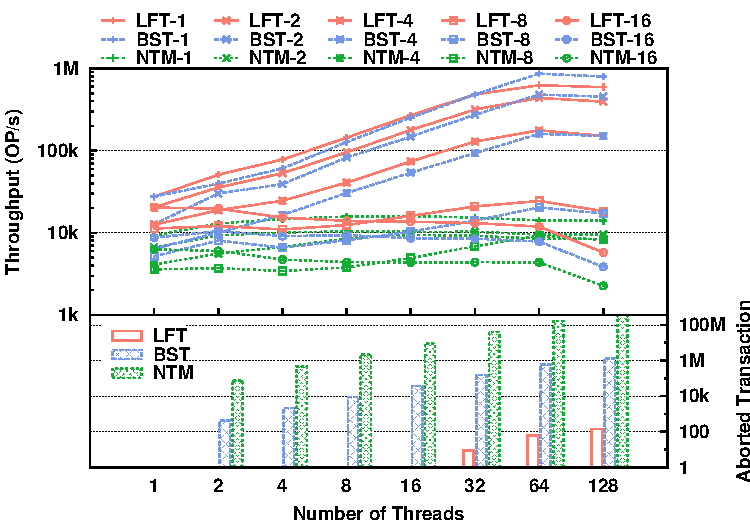
\includegraphics[width=1\columnwidth]{./data/amd50ins10kfilled.pdf}
        \caption{50\% \textsc{Insert}, 50\% \textsc{Delete}, 0\% \textsc{Find}}
        \label{fig:txnlist50}
    \end{subfigure}
	\hfill
    \begin{subfigure}{0.9\textwidth}
        \centering
        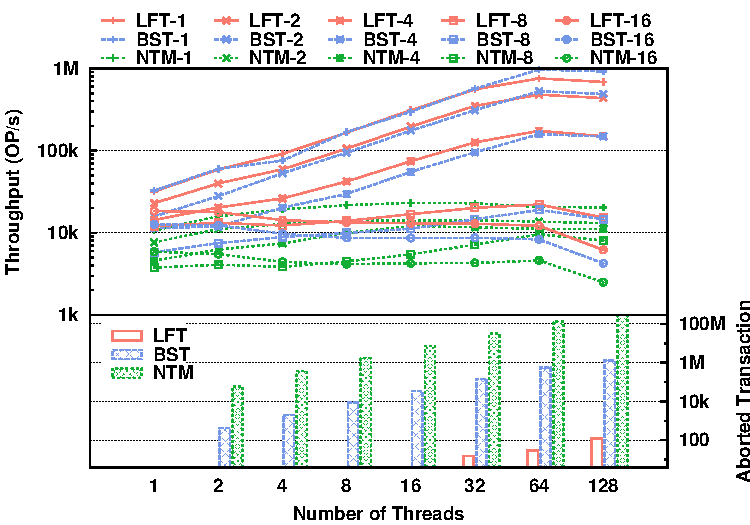
\includegraphics[width=1\columnwidth]{./data/amd33ins10kfilled.pdf}
        \caption{33\% \textsc{Insert}, 33\% \textsc{Delete}, 34\% \textsc{Find}}
        \label{fig:txnlist33}
    \end{subfigure}
\end{figure*}

\begin{figure*}[htbp]    
%	\hfill
	\ContinuedFloat
    \begin{subfigure}{0.9\textwidth}
        \centering
        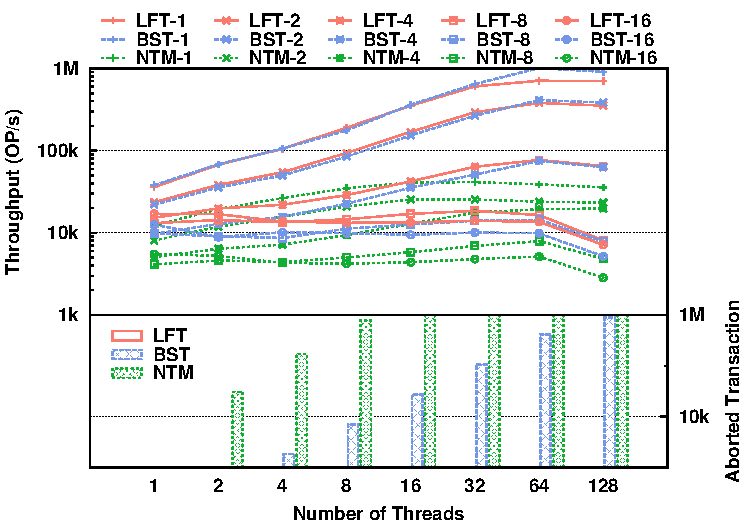
\includegraphics[width=1\columnwidth]{./data/amd15ins10kfilled.pdf}
        \vspace{-0.17in}
        \caption{15\% \textsc{Insert}, 5\% \textsc{Delete}, 80\% \textsc{Find}}
        \label{fig:txnlist15}
    \end{subfigure}
    \caption{Throughput and Spurious Abort Counts for Transaction Lists (10K Key Range)}
    \label{fig:txnlist}
\end{figure*}

\subsection{Transactional List}
\label{sec:txnlistexp}
We show the throughput and the number of spurious aborts in Figure~\ref{fig:txnlist} for all three types of lists.
The throughput is measured in terms of number of completed operations per second, which is the product of the number of committed transactions and transaction size.
The number of spurious aborts takes into account the number of aborted transactions except self-aborted ones (i.e., those that abort due to failed operations).
This is an indicator for the effectiveness of the contention management strategy.
Each thread performs $10^5$ transactions and the key range is set up to $10^4$.
Our lock-free transactional list is denoted by LFT, the boosted list by BST, and the NOrec STM list by NTM. 
The underlying list implementations for both LFT and BST were based on Harris' lock-free design~\cite{harris2001pragmatic}.
The linked list for NTM is taken directly from the benchmark implementation in RSTM suite.
Since the lock-free list and the RSTM list use different memory management scheme, we disable node reclamation for fair comparison of the synchronization protocols.
For each list legend annotation, we append a numeric postfix to denote the transaction size (e.g., BST-4 means the boosted list tested with 4 operations in one transaction). 

In Figure~\ref{fig:txnlist50}, threads perform solely write operations.
The upper half of the graph shows the throughput with both $y$- and $x$-axes in logarithm scale.
Starting with transaction of size 1, the throughput curve of BST-1 and LFT-1 essentially expose the overhead difference between the two transaction synchronization protocols.
Because each transaction contains only one operation, the code paths for transaction rollback in BST and transaction helping in LFT will not be taken.
For each node operation, BST-1 needs to acquire and release a mutex lock, while LFT-1 needs to allocate a transaction descriptor.
For executions within one CPU chip (no more than 16 threads), LFT-1 maintains a moderate performance advantage to BST-1, averaging more than 15\% speedup.
As the execution spawns across multiple chips, LFT-1's performance is setback by the use of descriptor, which incurs more remote memory accesses.
This trend can be observed for all scenarios with different transaction sizes.
Another noticeable trend is that LFT lists gain better performance as the transaction size grows.
For example, on 64 threads the throughput of LFT-2 slightly falls short behind that of BST-2, then the performance of LFT-4 is on par with BST-4, and finally LFT-8 and LFT-16 outperforms their BST counterpart by as much as 50\%.
Two factors contribute to the great scalability of LFT lists in handling large transactions: 1) its helping mechanism manages conflict and greatly reduces spurious aborts whereas in BST such aborts cause a significant amount of rollbacks; 2) the number of allocated transaction descriptors decreases as the transaction size grows whereas in BST the number of required lock acquisitions stays the same.

Generally, we observe that for small transaction sizes (no more than 4 operations), BST and LFT lists explore fine-grained parallelism and exhibit similar scalability trends.
The throughput increases linearly until 16 threads, and continues to increase at a slower pace until 64 threads.
Because executions beyond 16 threads span across multiple chips, the performance growth is slightly reduced due to the cost of remote memory accesses.
The executions are no longer fully concurrent beyond 64 threads, thus the overall throughput is capped and may even reduce due to context switching overhead.
LFT lists obtain an average of 25\% speedup over BST lists.
For large transactions, the throughputs of both LFT and BST list do not scale well.
This could be attributed to the semantic and the randomness of the benchmark.
As the transaction size grows, the probability of a randomly generated sequence of operations will all succeed is inherently smaller.
Most of the transactions were self-aborted due to some failed attempts to locate the target element.
LFT lists outperforms BST lists by an average of 40\% in these scenarios.
On the other hand, the throughput of all NTM lists stagnates as the number of threads increases.
Since NTM uses a single writer lock, concurrency is precluded for this write-dominated test case.
On 64 threads, both BST and LFT lists are able to achieve as much as 10 times better performance than NTM lists.

On the bottom half of Figure~\ref{fig:txnlist50}, we illustrate the histogram of spurious aborts across all transaction sizes and cluster them by thread counts.
The $y$-axis is in logarithmic scale.
For BST lists and NTM lists the number of spurious aborts grows linearly with the increase of threads.
BST lists have about 100 times less aborts than NTM lists, which matches our intuition that semantic conflict detection can remarkably reduce the number of false conflicts.
Also as expected no approach incurs spurious aborts in single thread scenario.
Remarkably, LFT lists do not introduce spurious aborts until 32 threads, and the number of aborts is 4 orders of magnitude smaller than that of BST lists. 
The helping mechanism of LFT is able to resolve majority of the conflicts in a cooperative manner, and aborts only when cyclic dependencies exist among transactions.

We show the results from mixed and read-dominated workloads in Figure~\ref{fig:txnlist33} and~\ref{fig:txnlist15}. 
The throughputs follow the same pattern as in Figure~\ref{fig:txnlist50} with LFT lists' performance advantage slightly diminishes in read-dominated workload.
This is because the \textsc{Find} operations in LFT lists also update descriptors in nodes, which requires extra cycles compared with read-only BST \textsc{Find} operations.
Nevertheless, LFT lists still maintain an average of 20\% speedup over BST lists in these scenarios and achieves as much as 40\% throughput gain for large transactions.  
Because of allowing reader concurrency, NTM lists also exhibit some degree of scalability in read-dominated scenarios.

\begin{figure*}[htbp]
	\begin{subfigure}{0.9\textwidth}
		\centering
		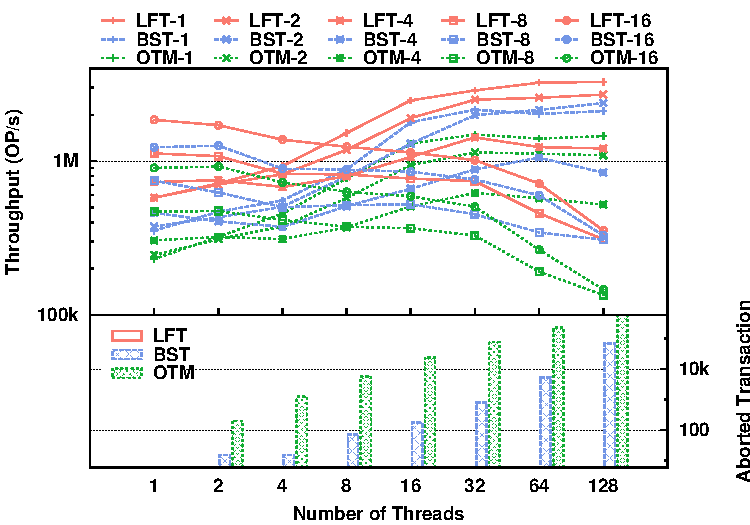
\includegraphics[width=1\columnwidth]{./data/amdskip50ins10kfilled.pdf}
		\caption{50\% \textsc{Insert}, 50\% \textsc{Delete}, 0\% \textsc{Find}}
		\label{fig:txnskip50}
	\end{subfigure}
	\hfill
	\begin{subfigure}{0.9\textwidth}
		\centering
		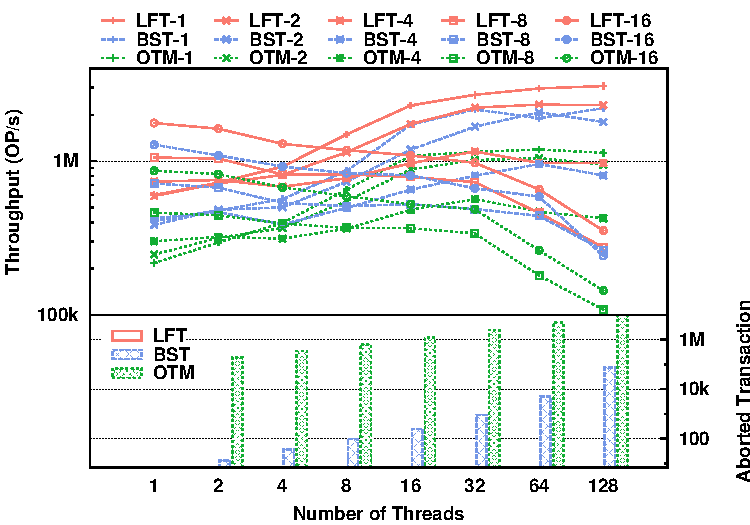
\includegraphics[width=1\columnwidth]{./data/amdskip33ins10kfilled.pdf}
		\caption{33\% \textsc{Insert}, 33\% \textsc{Delete}, 34\% \textsc{Find}}
		\label{fig:txnskip33}
	\end{subfigure}
\end{figure*}

\begin{figure*}[htbp]
%	\hfill
	\ContinuedFloat
	\begin{subfigure}{0.9\textwidth}
		\centering
		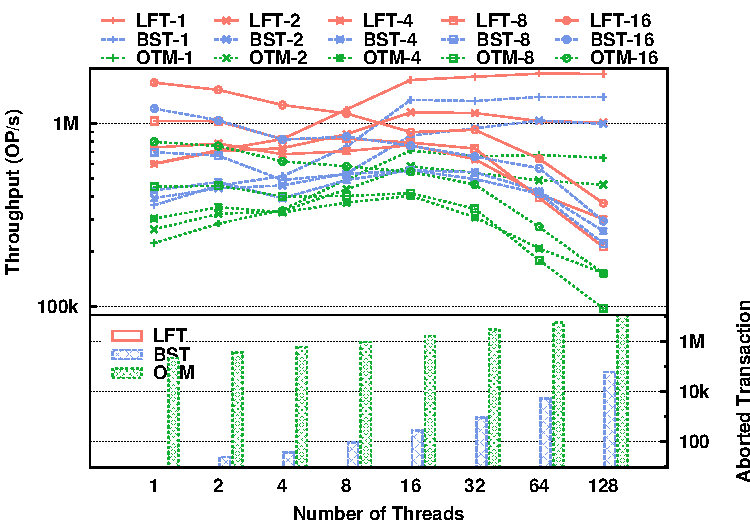
\includegraphics[width=1\columnwidth]{./data/amdskip15ins10kfilled.pdf}
		\vspace{-0.17in}
		\caption{15\% \textsc{Insert}, 5\% \textsc{Delete}, 80\% \textsc{Find}}
		\label{fig:txnskip15}
	\end{subfigure}
	\caption{Throughput and Spurious Abort Counts for Transaction Skiplists (1M Key Range)}
	\label{fig:txnskip}
\end{figure*}

\subsection{Transactional Skiplist}
\label{sec:txnskiplistexp}
In Figure~\ref{fig:txnskip}, we show the throughput and the number of spurious aborts for three types of transactional skiplists.
All of them are based on Fraser's open source lock-free skiplist~\cite{fraser2004practical}, and the epoch-based garbage collection is enabled in all three. 
The naming convention for BST and LFT skiplists remain the same as in Figure~\ref{fig:txnlist}.
We denote the STM based skiplist as OTM because it uses Fraser's object-based STM.
Compared with word-based STMs, an object-based STM groups memory into blocks thus reducing metadata overhead.
Since skiplists have logarithmic search time, we are able to stress the algorithms with heavier workloads: each threads now performs 1 million transactions and the key range is also boosted to 1 million.

Overall, with a peak throughput of more than 3 million (OP/s), transaction execution on skiplists is considerably more efficient than on linked lists.
Also both OTM and BST skiplists generates 2 orders or magnitude less spurious aborts than their list counterparts.
Because skiplist algorithms traverse exponentially less nodes than list algorithms, a single operation can finish much sooner, which greatly reduces the probability of memory access conflicts in STM and lock acquisition time out in transaction boosting.
Another noteworthy difference is that the divergent scalability trends of large and small transactions. 
As we can see in Figure~\ref{fig:txnskip50}, large transactions such as LFT-8 and LFT-16 achieves maximum throughputs on a single thread, then their throughputs steadily fall as the number of threads increases.
On the contrary, the throughputs of small transactions such as LFT-2 and LFT-4 start low, but gain momentum as more threads are added.
Large transactions have lower synchronization overhead but are vulnerable to conflict.
As the number of threads increases, a failed large transaction could easily forfeit a considerable amount of operations.
On the flip side, small transactions incur greater synchronization overhead, but are less likely to encounter conflicts when more threads contend with each other.
%Transaction lists also exhibits signs of such divergence in Figure~\ref{fig:txnlist} but it is not as significant.

Despite the differences, we still observe performance results generally similar to that of transaction lists.
LFT and BST skiplists outperform OTM skiplists by as much as 3 times across all scenarios, while LFT skiplists maintain an average of 60\% speedup over BST for large transactions.
For example, in Figure~\ref{fig:txnskip50} on 32 threads LFT-8 outperforms BST-8 by 125\%.
Even for small transactions, LFT skiplists begin to set the throughput apart from BST skiplists further than what is in Figure~\ref{fig:txnlist}.
For example, in Figure~\ref{fig:txnskip33} on 32 threads LFT-2 achieves an 30\% speedup over BST-2.



\begin{figure*}[htbp]
	\begin{subfigure}{0.9\textwidth}
		\centering
		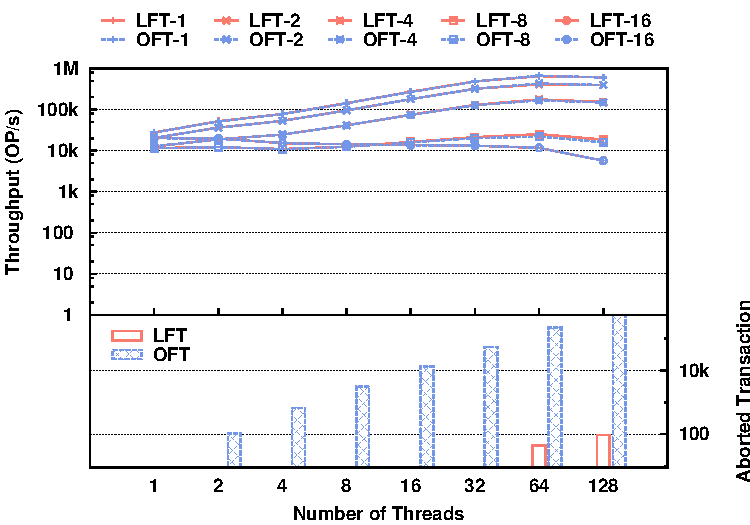
\includegraphics[width=1\columnwidth]{./data/oftlink50ins10kfilled.pdf}
		\caption{50\% \textsc{Insert}, 50\% \textsc{Delete}, 0\% \textsc{Find}}
		\label{fig:oftlist50}
	\end{subfigure}
	\hfill
	\begin{subfigure}{0.9\textwidth}
		\centering
		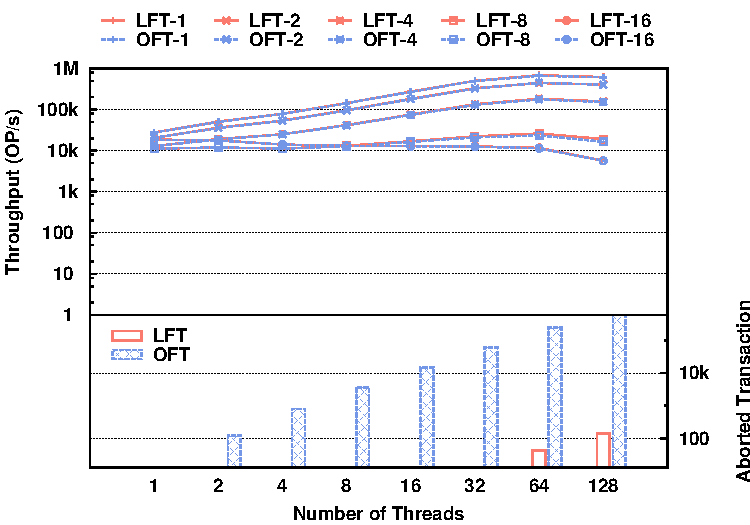
\includegraphics[width=1\columnwidth]{./data/oftlink33ins10kfilled.pdf}
		\caption{33\% \textsc{Insert}, 33\% \textsc{Delete}, 34\% \textsc{Find}}
		\label{fig:oftlist33}
	\end{subfigure}
\end{figure*}

\begin{figure*}[htbp]
%	\hfill
	\ContinuedFloat
	\begin{subfigure}{0.9\textwidth}
		\centering
		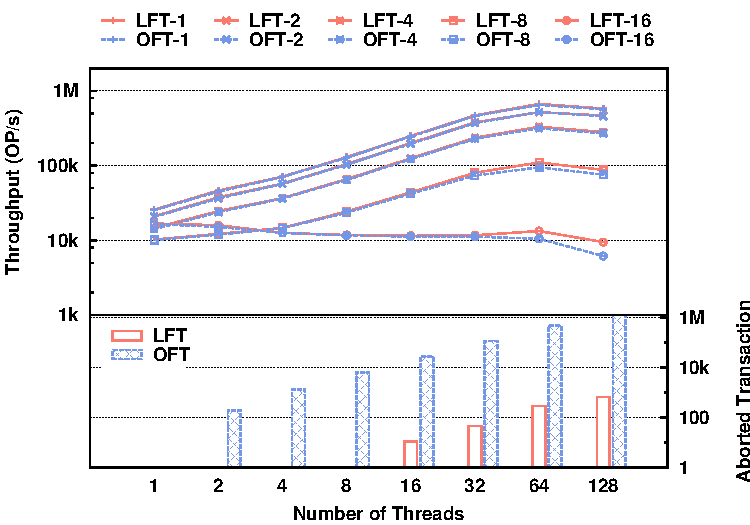
\includegraphics[width=1\columnwidth]{./data/oftlink15ins10kfilled.pdf}
		\vspace{-0.17in}
		\caption{15\% \textsc{Insert}, 5\% \textsc{Delete}, 80\% \textsc{Find}}
		\label{fig:oftlist15}
	\end{subfigure}
	\caption{Throughput and Spurious Abort Counts for Lock-free Versus Obstruction-free Transaction Lists (10K Key Range)}
	\label{fig:oftlist}
\end{figure*}




\begin{figure*}[htbp]
	\begin{subfigure}{0.9\textwidth}
		\centering
		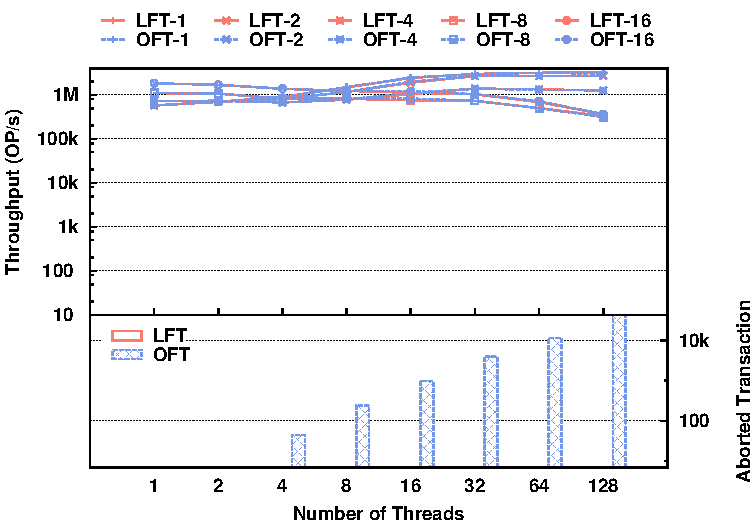
\includegraphics[width=1\columnwidth]{./data/oftskip50ins10kfilled.pdf}
		\caption{50\% \textsc{Insert}, 50\% \textsc{Delete}, 0\% \textsc{Find}}
		\label{fig:oftskip50}
	\end{subfigure}
	\hfill
	\begin{subfigure}{0.9\textwidth}
		\centering
		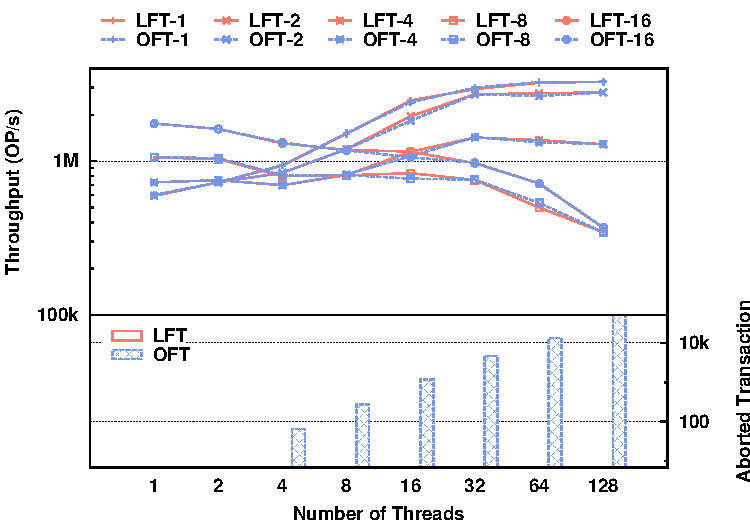
\includegraphics[width=1\columnwidth]{./data/oftskip33ins10kfilled.pdf}
		\caption{33\% \textsc{Insert}, 33\% \textsc{Delete}, 34\% \textsc{Find}}
		\label{fig:oftskip33}
	\end{subfigure}
\end{figure*}

\begin{figure*}[htbp]
%	\hfill
	\ContinuedFloat
	\begin{subfigure}{0.9\textwidth}
		\centering
		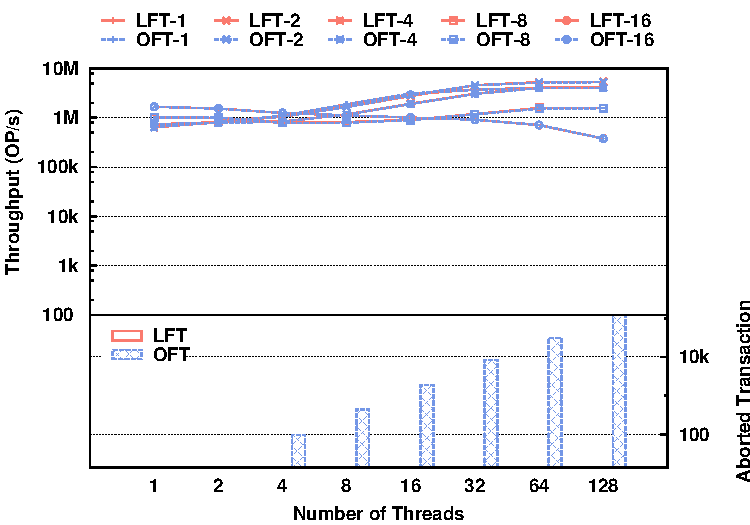
\includegraphics[width=1\columnwidth]{./data/oftskip15ins10kfilled.pdf}
		\vspace{-0.17in}
		\caption{15\% \textsc{Insert}, 5\% \textsc{Delete}, 80\% \textsc{Find}}
		\label{fig:oftskip15}
	\end{subfigure}
	\caption{Throughput and Spurious Abort Counts for Lock-free Versus Obstruction-free Transaction Skiplists (1M Key Range)}
	\label{fig:oftskip}
\end{figure*}

\subsection{Transactional Map}
In Figure~\ref{fig:map}, we show the throughput for the lock-free transactional map.
This map is a result of applying our approach to the wait-free hash map in~\cite{LaBorde2015}.

In order to test the transactional map with a large workload, we apply the same evaluation procedure as in Section~\ref{sec:txnskiplistexp}, giving each thread a workload of 1 million transactions and setting the key range to 1 million.
As we can see in Figure~\ref{fig:map50}, large transactions such as LFT-8 and LFT-16 achieve maximum throughput on a single thread, then their throughput steadily falls as the number of threads increases.
This is the same behavior observed in Figure~\ref{fig:txnskip50}.
The trend is weaker for the graph shown in Figure~\ref{fig:map15}, because the 75\% \textsc{Find} operations leads to a greater number of operations in the larger transaction sizes committing without failing.
An example of this is shown for the transaction size of 8 in  Figure~\ref{fig:map15}, which seems to level out compared to the other two operation distributions with the same transaction size.
Overall, with a peak throughput of more than 2.6 million (OP/s), transaction execution on hash maps is considerably more efficient than on linked lists, and comparable to skiplists despite the extra overhead on the \textsc{UpdateInfo} function due to the \textsc{Update} operation.
We do not show graphs of aborted transactions for the transactional map, because there were no spurious aborts for any tested scenario.

\begin{figure*}[htbp]
	\begin{subfigure}{0.8\textwidth}
		\centering
		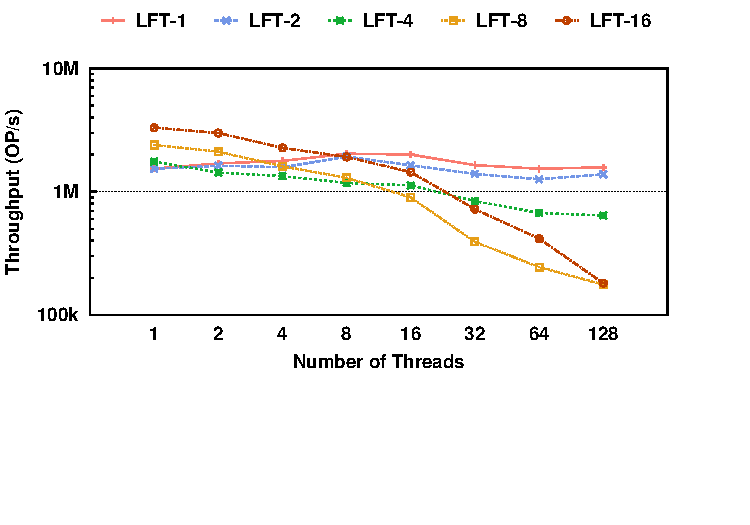
\includegraphics[trim=0 70 0 0,clip,width=1\columnwidth]{./data/map50ins.pdf}
		\caption{50\% \textsc{Insert}, 50\% \textsc{Delete}, 0\% \textsc{Update}, 0\% \textsc{Find} }
		\label{fig:map50}
	\end{subfigure}
	\hfill
	\begin{subfigure}{0.8\textwidth}
		\centering
		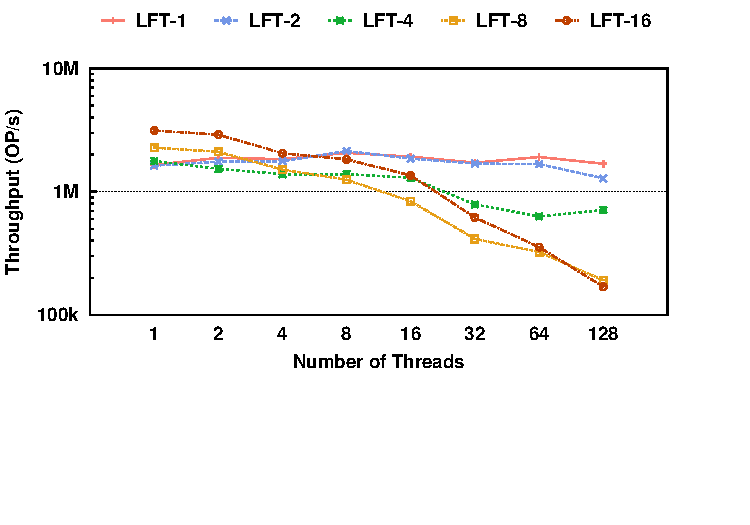
\includegraphics[trim=0 70 0 0,clip,width=1\columnwidth]{./data/map25ins.pdf}
		\caption{25\% \textsc{Insert}, 25\% \textsc{Delete}, 25\% \textsc{Update}, 25\% \textsc{Find}}
		\label{fig:map25}
	\end{subfigure}

	\begin{subfigure}{0.8\textwidth}
		\centering
		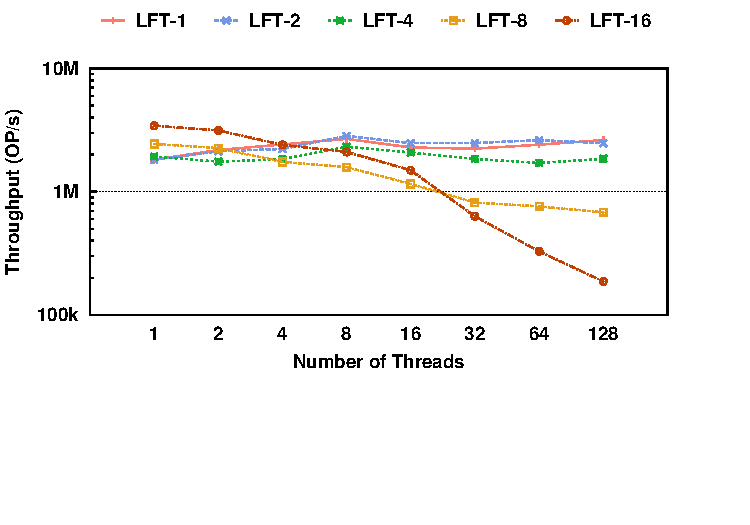
\includegraphics[trim=0 70 0 0,clip,width=1\columnwidth]{./data/map15ins.pdf}
		\vspace{-0.17in}
		\caption{15\% \textsc{Insert}, 5\% \textsc{Delete}, 5\% \textsc{Update}, 75\% \textsc{Find}}
		\label{fig:map15}
	\end{subfigure}
	\caption{Throughput for the Lock-free Transactional Hash Map (1M Key Range)}
	\label{fig:map}
\end{figure*}


\subsection{Obstruction-free Performance}
We compare the overhead and scalability of our obstruction-free version of transactional transformation against our lock-free version.
The lock-free version is denoted by LFT, and the obstruction-free version is denoted by OFT.

In Figure~\ref{fig:oftlist}, we show the throughput and the number of spurious aborts for the LFT list and the OFT list.
We apply the same evaluation procedure as in Section~\ref{sec:txnlistexp}, giving each thread a workload of $10^5$ transactions and setting the key range to $10^4$.
The OFT list performs similarly to the LFT list, with LFT outperforming OFT by merely 2\% on average.
However, with greater numbers of threads and larger transactions, OFT shows a performance disadvantage under higher contention.
For 64 and 128 threads, LFT-8 and LFT-16 achieve an average of 14\% speedup over OFT-8 and OFT-16.
These scenarios increase the chance that two transactions will concurrently access the same node.
In OFT, this situation will cause one of the transactions to spuriously abort, effectively canceling the progress that the aborted transaction made.
In contrast, the helping mechanism of LFT manages this conflict in a cooperative manner, allowing every transaction to make progress.

In Figure~\ref{fig:oftskip}, we compare the performance of the OFT skiplist to the LFT skiplist.
As in Section~\ref{sec:txnskiplistexp}, we boost the workload to 1 million transactions per thread and increase the key range to 1 million.
Because of the larger key range, the number of spurious aborts is greatly reduced.
As a result, the OFT skiplist does not show the same performance disadvantage as the OFT list.
In this low-contention environment, the LFT and OFT skiplists perform very similarly, only showing slight variations in throughput.

\section{Related Work}
\label{sec:related}
Non-blocking linked data structures have been extensively studied because their distributed memory layout provides data access parallelism and scalability under high levels of contention~\cite{harris2001pragmatic,linden2013skiplist,zhang2015lockfree,michael2002high}.
To the best of our knowledge, there is no existing linked data structure that provides native support for transactions.
A transactional execution of data structure operations can be seen as a restricted form of \emph{software transactions}~\cite{harris2010transactional}, in which the memory layout and the semantics of the operations are well defined according to the specification of the data structure. 
Straightforward generic constructions can be implemented by executing all shared memory accesses in coarse-grained \emph{atomic sections}, which can employ either optimistic (e.g., STM) or pessimistic (e.g., lock inference) concurrency control.
More sophisticated approaches~\cite{bronson2010transactional,herlihy2008transactional,golan2015automatic} exploit semantic conflict detection for transaction-level synchronization to reduce benign conflicts.
We draw inspirations from previous semantic based conflict detection approaches.
However, with the specific knowledge on linked data structure, we further optimize the transaction execution by performing in-place conflict detection and contention management on existing nodes.
%In our work, we combine both fine-grained thread-level synchronization found in existing lock-free data structures and semantic conflict detection to implement transactional linked data structures without the overhead of atomic section synchronizations.

\subsection{Transactional Memory}
Initially proposed as a set of hardware extensions by Herlihy and Moss~\cite{herlihy1993transactional}, transactional memory was intended to facilitate the development of lock-free data structures.
%Even with Intel's recent release of commercial support of best-effort hardware transaction memory (HTM) in their Haswell processors, 
However, due to current HTM's cache-coherency based conflict detection scheme, transactions are subject to spurious failures during page faults and context switches~\cite{dice2009early}.
%This along with excessive aborts under moderate contention~\cite{christina2015resource} make HTM less desirable for implementing transactions in non-blocking data structures.
This makes HTM less desirable for data structure implementations.
Considerable amount of work and ingenuity has instead gone into designing lock-free data structures using low-level synchronization primitives such as \textsc{CompareAndSwap}, which empowers researchers to devise algorithm-specific fine-grained concurrency control protocol.

The first software transactional memory was proposed by Shavit and Touitou~\cite{shavit1997software}, which is lock-free but only supports a static set of data items.
Herlihy, et al., later presented DSTM~\cite{herlihy2003software} that supports dynamic data sets on the condition that the progress guarantee is relaxed to obstruction-freedom.
Over the years, a large number of STM implementations have been proposed~\cite{saha2006mcrt,fraser2004practical,marathe2006lowering,dice2006transactional,dalessandro2010norec}.
We omit complete reviews because it is out of the scope of this paper.
As more design choices were explored~\cite{marathe2004design}, we have seen emerging discussions on the issues of STM regarding usability~\cite{Rossbach2010transactional}, performance~\cite{cascaval2008software}, and expressiveness~\cite{guerraoui2008obstruction}.
There is also an increasing realization that the read/write conflicts inherently provide insufficient support for concurrency when shared objects are subject to contention~\cite{koskinen2010coarse}.
It has been suggested that ``STM may not deliver the promised efficiency and simplicity for \emph{all} scenario, and multitude of approaches should be explored catering to different needs''~\cite{attiya2010inherent}.
%Unlike STM-based data structures, our approach eliminate false conflict and excessive aborts by adopting semantic conflict detection.

%Kempf2014combining combines lock inference and stm.
\subsection{Lock Inference}
STM implementations are typically \emph{optimistic}, which means they execute under the assumption that interferences are unlikely to occur.
They maintain computationally expensive redo or undo logs to allow replay or rollback in case a transaction experiences interference.
In light of this shortcoming, pessimistic alternatives based on lock inference have been proposed~\cite{mccloskey2006autolocker}.
These algorithms synthesize enough locks through static analysis to prevent data races in atomic sections.
The choice of locking granularity has an impact on the trade-off between concurrency and overhead.
Some approaches require programmers' annotation~\cite{golan2013concurrent} to specify the granularity, others automatically infer locks at a fixed granularity~\cite{emmi2007lock} or even multiple granularities~\cite{cherem2008inferring}.
Nevertheless, most approaches associate locks with memory locations, which may lead to reduced parallelism due to false conflicts as seen in STM. 
Applying these approaches to real-world programs also faces scalability changes in the presence of large libraries ~\cite{gudka2012lock} because of the high complexity involved in the static analysis process.
%Applying these approaches to real-world programs also faces scalability changes in the presence of large libraries ~\cite{gudka2012lock} because of the high cyclomatic complexity~\footnote{A measure of the number of linearly independent execution paths~\cite{mccabe1976complexity}.} involved in the static analysis process.
Moreover, the use of locks degrades any non-blocking progress guarantee one might expect from using a non-blocking library.
%In contrast, our approach guarantees lock-free progress.

\subsection{Semantic Conflict Detection}
Considering the imprecise nature of data-based conflict detection, semantic-based approaches have been proposed to identify conflicts at a high-level (e.g., two commutative operations would not raise conflict even though they may access and modify the same memory data) which enables greater parallelism.
Because semantically independent transactions may have low-level memory access conflicts, some other concurrency control protocol must be used to protect accesses to the underlying data structure.
This results in a two-layer concurrency control.
Transactional boosting proposed by Herlihy~\cite{herlihy2008transactional} is the first dedicated treatment on building highly concurrent transactional data structures using a semantic layer of abstract locks. 
%Transactional boosting~\cite{herlihy2008transactional} is a semantic-based methodology for transforming linearizable concurrent data structures into transactional data structures.
The idea behind boosting is intuitive: if two operations commute they are allowed to proceed without interference (i.e., thread-level synchronization happens within the operations); otherwise they need to be synchronized at the transaction level.
It treats the base data structure as a black box and uses \emph{abstract locking} to ensure that non-commutative method calls do not occur concurrently. 
For each operation in a transaction, the boosted data structure calls the corresponding method of the underlying linearizable data structure after acquiring the abstract lock associated with that call. 
%In the boosted linked list shown in Figure~\ref{fig:boosting}, the abstract lock is pertaining to each key.  
%Thread 1 tries to execute \textsc{Insert(1)} and \textsc{Insert(4)} in a transaction while Thread 2 tries to execute \textsc{Remove(9)} and \textsc{Insert(4)} transactionally.
A transaction aborts when it fails to acquire an abstract lock, and it recovers from failure by invoking the inverses of already executed calls. 
Its semantic-based conflict detection approach eliminates excessive false conflicts associated with STM-based transactional data structures, but it still suffers from performance penalties due to the rollbacks of partially executed transactions.
Moreover, when applied to non-blocking data structures, the progress guarantee of the boosted data structure is degraded because of the locks used for transactional-level synchronization.
Transactional boosting is pessimistic in that it acquires locks eagerly before the method calls, but it still requires operation rollback because not all locks are acquired at once.
%PTB, black box design, forfiet data structure specific optimization, need to reverse operation upon failure
Koskinen et al.~\cite{koskinen2010coarse} later generalized this work and introduce a formal framework called coarse-grained transactions.
Bronson et al. proposed transaction prediction, which maps the abstract state of a set into memory blocks called predicate and relies on STM to synchronize transactional accesses~\cite{bronson2010transactional}.
Hassan et al.~\cite{hassan2014developing} proposed an optimistic version of boosting, which employs a white box design and provides throughput and usability benefits over the original boosting approach.
Other STM variants, such open nested transactions~\cite{ni2007open} support a more relaxed transaction model that leverages some semantic knowledge based on programmers' input.
The relaxation of STM systems and its implication on composability have been studied by Gramoli et al.~\cite{gramoli2013composing}.
The work by Golan-Gueta et al.~\cite{golan2015automatic} applies commutativity specification obtained from programmers' input to inferring locks for abstract data types.

Spiegelman, et al.~\cite{spiegelman2016transactional} propose an approach that collects a read-set and write-set for a transaction and performs validation on the nodes before executing physical modifications.
When a transaction begins, it is assigned a version number.
The transaction then collects a local read-set of nodes that it reads and a write-set of nodes that it will modify.
At commit-time, the transaction locks the nodes in the write-set, and then it validates that all nodes in the read-set are unchanged by checking their version numbers.
If the transaction fails to acquire a lock or the validation fails, that means another transaction made non-commutative method calls, and the transaction aborts.
If successful, the transaction makes physical modifications to the nodes in the write-set, updates the nodes' version numbers, and then releases the locks.
This approach benefits from the absence of rollbacks, but when applied to non-blocking data structures, it diminishes the progress guarantee of the data structure by using locks.
This problem could be remedied by replacing locks with transaction descriptors, and we could ensure opacity by applying a helping mechanism similar to the one used in our approach.
However, to prevent the livelock scenario mentioned in Section~\ref{sec:txnexec}, we must detect cyclic dependencies among transactions and abort one of the transactions when a cyclic dependency occurs.
The aborted transaction would then need to perform a rollback of the changes it made, which would incur a performance penalty.
We do not compare our approach to theirs as their source code is proprietary~\cite{Spiegelman2016b}.

\section{Conclusion}
\label{sec:conclusion}
We introduced a methodology for transforming lock-free linked data structures into high-performance lock-free transactional data structures. 
Our approach embeds the transaction metadata in each node, which enables resolving transaction conflicts cooperatively through thread-level synchronization.
No undo logs nor rollbacks are needed because operations can correctly interpret the logical status of nodes left over by aborted transactions.
Data structures that guarantees lock-free or weaker progress will be able to maintain their progress properties during the transformation.
We demonstrated the application of our lock-free transactional transformation on two fundamental data structures: a linked list and a skiplist.  
%TODO: speedup
The performance evaluation results show that our transaction synchronization protocol has low overhead and high scalability--providing an average of $40\%$ speed-up over our good-faith transaction boosting implementations across all scenarios and as much as $125\%$ more throughput for large transactions.
The performance gain over STMs are even more substantial: more than 10 times over the alternative word-based STM and 3 times over the object-based STM.
Besides the performance advantages, our approach decreases spurious aborts to a minimum, which is desirable because transaction success rate is a decisive factor for a majority of the applications.

We also presented an obstruction-free version of our algorithm which can be applied to dynamic execution scenarios, and an example of our approach using map data structures.

We defer describing the methodology to encompass dictionary API to future work.
The key change is to add two value fields (old, and current) in the \textsc{NodeInfo} structure so that the old version can be recovered if update fails.
We also plan to further evaluate our approach on SMP systems to verify potential performance gains under low memory latency.

%\begin{figure*}[p]
    %\centering
    %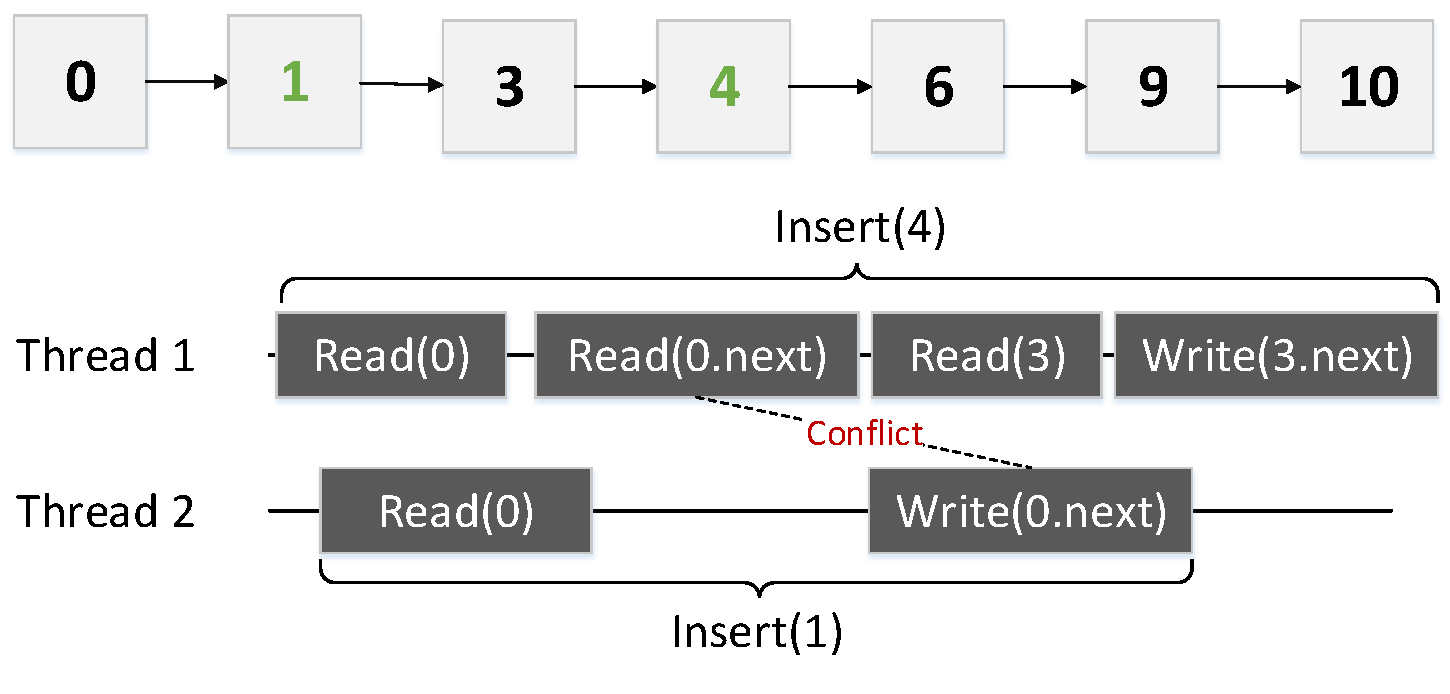
\includegraphics[width=0.9\textwidth]{figure/stmconflict.pdf}
    %\caption{False Conflict in STM}
    %\label{fig:stmconflict}
%\end{figure*}

%\begin{figure*}[p]
    %\centering
    %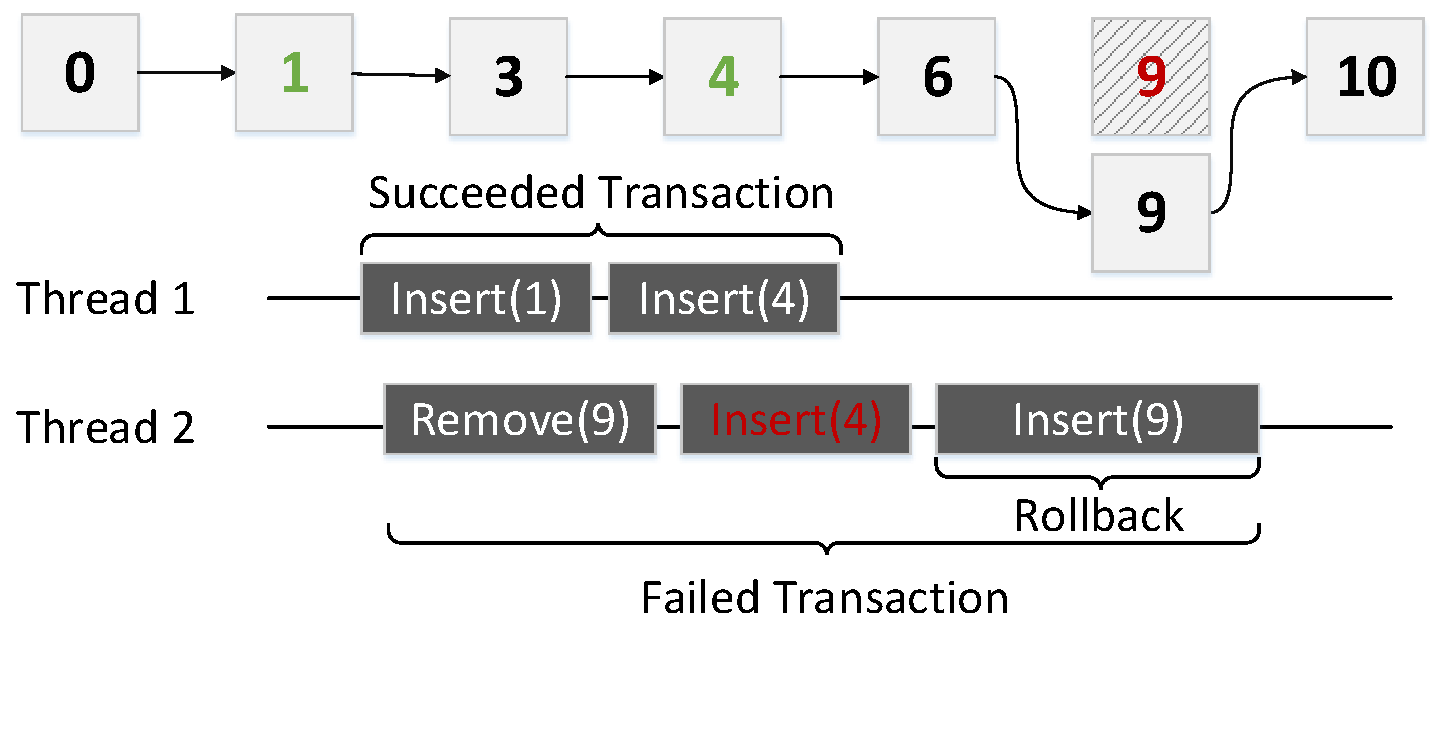
\includegraphics[width=0.9\textwidth]{figure/boosting.pdf}
    %\caption{Rollbacks in Transactional Boosting}
    %\label{fig:boosting}
%\end{figure*}


% Appendix
%\appendix
%\section*{APPENDIX}
%\setcounter{section}{1}
%
%
%\appendixhead{ZHOU}
%
%% Acknowledgments
%\begin{acks}
% This work is supported by the National Science Foundation under ACI Award No. 1440530.
%\end{acks}

% Bibliography
%\FloatBarrier %usepackage{placeins}
\bibliographystyle{ACM-Reference-Format-Journals}
\bibliography{citation}


\end{document}
